\documentclass[11pt]{article}

\usepackage[letterpaper, margin=1in]{geometry}

\usepackage[spanish]{babel}
\usepackage[utf8]{inputenc}
\usepackage{multirow}
\usepackage{tabularx}
\usepackage{longtable}
\usepackage[colorlinks=true,urlcolor=blue,linkcolor=black,citecolor=red]{hyperref}     % Para insertar hipervínculos y marcadores


%Figuras
\usepackage{graphicx, subfigure}
\usepackage[]{tikz}
\usepackage{pbox}

%Matemática
\usepackage{amsmath}
\usepackage{amssymb}

% Símbolos mate extra (alfabetos, etc.)
\usepackage{mathrsfs}


%Algoritmos
\usepackage{float}
\usepackage{algorithm}
\usepackage{algorithmicx}
\usepackage{algpseudocode}
\usepackage{listings}
\lstset{language=C++,basicstyle=\ttfamily,numbers=left}
\usepackage{minted}

\usepackage{color}
\usepackage{xcolor,colortbl}
\usepackage{hyperref}
\usepackage{adjustbox}
\usepackage{multirow}
\usepackage{multicol}
\usepackage{epsfig}
\usepackage{mdframed}
\usepackage{tcolorbox}
\usepackage{booktabs}
\usepackage{tabulary}
\usepackage{pdfpages}
\numberwithin{figure}{section}
\numberwithin{equation}{section}
\numberwithin{table}{section}

%Define color
\definecolor{darkblue}{rgb}{0 , 0.054 , 0.196}
\definecolor{verdito}{rgb}{0.6,1,0.6}
\definecolor{bl}{rgb}{0.6602, 0.796875, 0.8862}
\definecolor{cl}{rgb}{0.8359, 0.9140625, 0.96875}
\definecolor{bg}{rgb}{0.95,0.95,0.95}
\definecolor{p1}{rgb}{1.0,0.698,0.4}
\definecolor{gray97}{gray}{.97}
\definecolor{gray75}{gray}{.75}
\definecolor{gray45}{gray}{.45}
\definecolor{LightGreen}{rgb}{0.8,1,0.8}
\definecolor{DarkGreen}{rgb}{0.2,0.6,0.3}
\definecolor{lightgray}{gray}{0.9}
\definecolor{bg1}{rgb}{0.8,1.0,0.8}

%Unidades Matemáticas 
\usepackage{unitsdef}	  
\renewcommand{\unitvaluesep}{\hspace*{2pt}}

\title{ \Large \underline{ \textbf{Reporte de Laboratorio 4: Programación genérica}}}
\author{ $\rightarrow$ David Elizondo Garro, [B32359]\\ 
		 $\rightarrow$ José Adrián Sanabria Roselló, [B46420]\\ 
         $\rightarrow$ José Pablo Martínez Hernández, [B34024]\\
         {\small \textbf{Subgrupo 3}}}

\begin{document}

\maketitle
\hrule
\hrule
\tableofcontents
\hspace{5mm}
\hrule
\hrule


%%%%%%%%%%%%%%%%%%
%--> LABORATORIO 1
%%%%%%%%%%%%%%%%%%
%\section{Introducción}
Esta es la introducción
\subsection{Objetivos}
Texto grande:
\begin{huge}
Hacer una demostración.
\end{huge}

\subsubsection{Listas}
Lista con viñetas:
\begin{itemize}
\item Ob1.
\item Ob2.
\end{itemize}

Lista numerada:
\begin{enumerate}
\item No 1.
\item No 2.
\end{enumerate}

\section*{Sección no numerada}
Fin de sección.

\section{Matemática básica}

\subsection{Fundamentos}
Símbolos entre el texto: $a^2 + b^2 = c^2$.

Función definida por casos:
\begin{equation}
f(x) = %
\begin{cases}
	1	& \text{Si } x > 0 \\
	-1	& \text{Si } x < 0 \\
	0   & \text{Si } x = 0
\end{cases}
\end{equation}

Potencias y raíces:
\begin{equation}
\sqrt{b^2 - 4ac}
\end{equation}

Fracciones
\begin{equation}
\frac{a^2}{(b + c)^2} + \frac{1}{n}
\end{equation}

Agrupadores de tamaño variable:
\begin{equation}
\Big[ \Big( \frac{1}{n} + x^2 \Big) - k\big(x + 1\big)^3 \Big]
\end{equation}

Matrices (como ecuación no numerada):
\begin{equation*}
 \left(
    \begin{array}{ccc}
        a & b & c \\
        d & e & f \\
        g & h & i
    \end{array}
\right)
\end{equation*}

Ambiente ``ecuación'' con sumatoria (promedio):
\begin{equation}
\bar{x} = \frac{1}{n} \sum_{i=1}^{n} x_i
\label{media}
\end{equation}

Ambiente ``ecuación'' con integral:
\begin{equation}
\int _a ^b f(x) dx
\end{equation}

\subsection{Ejemplos de símbolos y constantes}

Volumen de una esfera:
\begin{equation}
\frac{4}{3} \pi r^3
\end{equation}

Regla trapezoidal uniforme:
\begin{equation}
\int_a ^b f(x)dx \approx \sum_{k=1}{N} \big( f(x_{k+1}) + f(x_k) \big)
\end{equation}

Varianza:
\begin{equation}
\sigma^2 = \frac{1}{N} \sum_{i=1}^{N} (x_i - \mu)^2
\end{equation}

donde $\mu$ es la media definida en \ref{media}.
\newline

Y otros símbolos:
\begin{itemize}
\item Derivadas parciales: $\dfrac{\partial f}{\partial x}$

\item Letras griegas: $\alpha, \beta, \gamma, \Gamma, \delta, \Delta, \sigma, \Sigma, \ldots$.

\item Fórmulas: $\forall x\exists y ~|~ x \in C \land y \in A \cap B$, $\nexists n ~|~ N \cup \{n\} = \emptyset$

\item Símbolos adicionales: $\mathbb{Z}, \mathbb{N}, \mathbb{R}$

\item Y más: $\mathscr{A}, \mathscr{B}, \mathscr{Z}$
\end{itemize}

\section{Imágenes y figuras}


Figura centrada:
\begin{figure}[ht]
\centering

\includegraphics[scale=0.8]{imgL1/cosme.jpg}
\caption{Cosme Fulanito}
\label{fig:cosme}
\end{figure}
La figura \ref{fig:cosme} muestra al destacado autor de este trabajo.

Imagen a la derecha:

\begin{flushright}

\includegraphics[scale=0.5]{imgL1/cosme.jpg}
\end{flushright}




\section{Tablas}
Tablita:

\begin{table}[ht]
\begin{center}
    \begin{tabular}{ c | c | c }
        1 & 2 & 3 \\ 
        \hline 
        4 & 5 & 6 \\  
        7 & 8 & 9    
    \end{tabular}
\end{center}
\caption{Tabla pequeña}
\end{table}
tabla larga partida en paginas:\\


\begin{longtable}{|c|c|c|c|}
        \hline
        \textbf{$\Delta \tau$ (píxeles)} & \textbf{$\Delta \rho$ (píxeles)} & \textbf{$\Delta \phi$ (grados)} & \textbf{Clasificador} \\  
        \hline
        \endhead
        1 & 1 & 0,5 & K-Means \\ \hline
        1 & 1 & 0,5 & SMO \\ \hline
        1 & 1 & 0,5 & LogitBoost \\ \hline
        \ldots & ... & ... & ... \\ \hline
        1 & 1 & 1 & K-Means \\ \hline
        1 & 1 & 1 & SMO \\ \hline
        ... & ... & ... & ... \\ \hline
        1 & 1 & 2 & K-Means \\ \hline
        1 & 1 & 2 & SMO \\ \hline
        ... & ... & ... & ... \\ \hline
        3 & 3 & 2 & BayesNet \\ \hline
        1 & 1 & 0,5 & K-Means \\ \hline
        1 & 1 & 0,5 & SMO \\ \hline
        1 & 1 & 0,5 & LogitBoost \\ \hline
        ... & ... & ... & ... \\ \hline
        1 & 1 & 1 & K-Means \\ \hline
        1 & 1 & 1 & SMO \\ \hline
        ... & ... & ... & ... \\ \hline
        1 & 1 & 2 & K-Means \\ \hline
        1 & 1 & 2 & SMO \\ \hline
        ... & ... & ... & ... \\ \hline
        3 & 3 & 2 & BayesNet \\ \hline
        1 & 1 & 0,5 & K-Means \\ \hline
        1 & 1 & 0,5 & SMO \\ \hline
        1 & 1 & 0,5 & LogitBoost \\ \hline
        ... & ... & ... & ... \\ \hline
        1 & 1 & 1 & K-Means \\ \hline
        1 & 1 & 1 & SMO \\ \hline
        ... & ... & ... & ... \\ \hline
        1 & 1 & 2 & K-Means \\ \hline
        1 & 1 & 2 & SMO \\ \hline
        ... & ... & ... & ... \\ \hline
        3 & 3 & 2 & BayesNet \\ \hline
        1 & 1 & 1 & K-Means \\ \hline
        1 & 1 & 1 & SMO \\ \hline
        ... & ... & ... & ... \\ \hline
        1 & 1 & 2 & K-Means \\ \hline
        1 & 1 & 2 & SMO \\ \hline
        ... & ... & ... & ... \\ \hline
        3 & 3 & 2 & BayesNet \\ \hline
        1 & 1 & 0,5 & K-Means \\ \hline
        1 & 1 & 0,5 & SMO \\ \hline
        1 & 1 & 0,5 & LogitBoost \\ \hline
        ... & ... & ... & ... \\ \hline
        1 & 1 & 1 & K-Means \\ \hline
        1 & 1 & 1 & SMO \\ \hline
        ... & ... & ... & ... \\ \hline
        1 & 1 & 2 & K-Means \\ \hline
        1 & 1 & 2 & SMO \\ \hline
        ... & ... & ... & ... \\ \hline
        3 & 3 & 2 & BayesNet \\ \hline
        1 & 1 & 1 & K-Means \\ \hline
        1 & 1 & 1 & SMO \\ \hline
        ... & ... & ... & ... \\ \hline
        1 & 1 & 2 & K-Means \\ \hline
        1 & 1 & 2 & SMO \\ \hline
        ... & ... & ... & ... \\ \hline
        3 & 3 & 2 & BayesNet \\ \hline
        1 & 1 & 0,5 & K-Means \\ \hline
        1 & 1 & 0,5 & SMO \\ \hline
        1 & 1 & 0,5 & LogitBoost \\ \hline
        ... & ... & ... & ... \\ \hline
        1 & 1 & 1 & K-Means \\ \hline
        1 & 1 & 1 & SMO \\ \hline
        ... & ... & ... & ... \\ \hline
        1 & 1 & 2 & K-Means \\ \hline
        1 & 1 & 2 & SMO \\ \hline
        ... & ... & ... & ... \\ \hline
        3 & 3 & 2 & BayesNet \\ \hline
        
    
    \caption{Grupos estudiados en el experimento B.}
    \label{tab:gruposB}
\end{longtable}

\section{Uso de referencias bibliográficas}
Para citar trabajos se utiliza la instrucción \textbf{cite} \cite{Bonaparte75}.

Dos o más se pueden separar por coma \cite{Brown, Fulanito1999}.

%%%%%%%%%%%%%%%%%%
%--> LABORATORIO 2
%%%%%%%%%%%%%%%%%%
%\section{Introducción}
En este laboratorio se realizó un programa que simula el comportamiento del código genético, es decir, la traducción de una secuencia de nucleótidos en el ARN, a una secuencia de aminoácidos, tal y como sucede en los seres vivos. La secuencia de ARN es caracterizada por cuatro bases nitrogenadas, representadas con las letras A, G, C y U (adenina, guanina, citosina y uracilo, respectivamente). Estos nucleótidos se agrupan de 3 en 3, grupos que se denominan codones, y cada codón se traduce en un aminoácido. Existen 3 codones especiales que no se traducen en aminoácidos, sino que marcan el inicio y final de una cadena.

El funcionamiento del presente programa se basa en un archivo de origen (\texttt{.txt}) en el cual se encuentran las cadenas de nucleótidos, una serie de métodos que se encargan de la traducción y, finalmente, la escritura de la cadena de aminoácidos resultante en un archivo de destino. Se crea una clase llamada FILEUTIL que, haciendo uso de la librería \texttt{fstream} de C++, se encarga de las operaciones de apertura, lectura y escritura de los archivos; y una clase TRANSLATOR que lleva a cabo todo el proceso de traducción.


\subsection{Objetivos}
\begin{enumerate}
\item Familiarizarse con el lenguaje de programación C++ y el paradigma de orientación a objetos.
\item Resolver un problema mediante el uso de arreglos, funciones, clases y memoria dinámica.
\item Practicar el uso de makefiles, la documentación con Doxygen y el control de versiones en GitLab.
\item Utilizar las herramientas de manejo de archivos de C++.
\end{enumerate}

\section{Enunciado}
Escriba y documente (con Doxygen) un programa en C++, usando orientación a objetos, que genere los aminoácidos a partir de los codones de un código genético (ARN) cualquiera. Para esto,
el programa recibe de la línea de comandos dos rutas, el archivo de entrada y el archivo de salida.\\
El archivo de entrada estará compuesto por una serie de bases nitrogenadas (A, G, C, U) múltiplo de 3, que siempre empieza y termina por un codón de parada.\\
Archivo de entrada con múltiples línea de datos.\\
En archivo de salida estarán los aminoácidos que se traducen a partir de las bases nitrogenadas.
Use la figura \ref{fig:1} o \url{https://en.wikipedia.org/wiki/Genetic_code#RNA_codon_table}.

\begin{figure}[H]
\centering
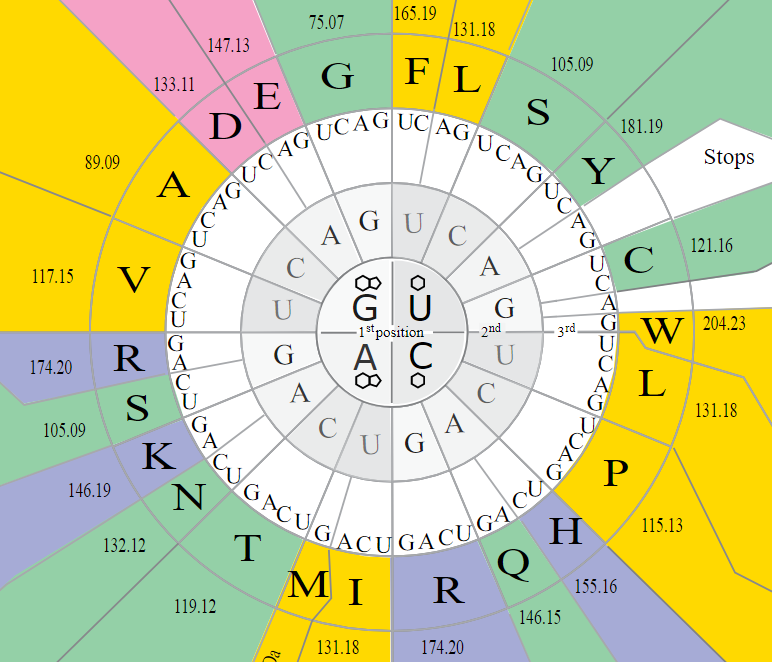
\includegraphics[width=0.6\textwidth]{imgs/Labo2/cod-gen}
\caption{Tabla de conversión ARN a aminoácido}
\label{fig:1}
\end{figure}

\subsection{Ejemplo 1}
El siguiente archivo de entrada:
\begin{lstlisting}[backgroundcolor=\color{verdito}]
UAACCUUCUACUACGUAG
\end{lstlisting}
Produce el siguiente archivo de salida:
\begin{lstlisting}[backgroundcolor=\color{verdito}]
PSTT
\end{lstlisting}

\subsection{Ejemplo 2}
El siguiente archivo de entrada:
\begin{lstlisting}[backgroundcolor=\color{verdito}]
UAACCUUCUACUACGUAG
UAGUCUCCUACGACUUUA
UAACCUUCUACUACGUAG
UAGUCUCCUACGACUUUA
\end{lstlisting}
Produce el siguiente archivo de salida:
\begin{lstlisting}[backgroundcolor=\color{verdito}]
TTPS
SPTT
TTPS
SPTT
\end{lstlisting}

\subsection{Detalles}
Cree al menos dos clases \texttt{Translator} y \texttt{FileUtil}. Los métodos mínimos para ambas clases se muestran en las tablas \ref{T1} y \ref{T2}. Además desarrolle la función \texttt{main} en un archivo aparte.


\begin{table}[H]
\begin{center}
    \begin{tabular}{ |c|c|c|c| }
    	\hline
    	\cellcolor{cl} \textbf{Tipo de retorno} & \cellcolor{cl} \textbf{Nombre del método} & \cellcolor{cl} \textbf{Argumentos} & \cellcolor{cl} \textbf{Detalle}\\ \hline \hline
         & Translator &   & Método constructor\\  \hline
         & $\sim$Translator & & Método destructor\\ \hline
         string & translate & string s & Método que traduce 1 string s\\ & & & en otro string usando las\\ & & & reglas del código genético\\ \hline
         string* & translate & string* s, int n & Método que traduce n strings\\ & & & s en otros usando las reglas\\ & & &  del código genético\\ \hline
    \end{tabular}
\end{center}
\label{T1}
\caption{Métodos de la clase \texttt{Translator}}
\end{table}


\begin{table}[H]
\begin{center}
    \begin{tabular}{ |>{\centering\arraybackslash}m{3.5cm}|>{\centering\arraybackslash}m{3.9cm}|>{\centering\arraybackslash}m{3cm}|>{\centering\arraybackslash}m{5cm}| }
    	\hline
    	\cellcolor{cl} \textbf{Tipo de retorno} & \cellcolor{cl} \textbf{Nombre del método} & \cellcolor{cl} \textbf{Argumentos} & \cellcolor{cl} \textbf{Detalle}\\ \hline \hline
         & FileUtil & string s, io\_base::openmode p & Método constructor, usa el archivo indicado por la ruta s\\ \hline
         & $\sim$FileUtil  & & Método destructor\\ \hline
         string & read & & Método que lee una línea del
\\ & & & archivo asociado al objeto\\ \hline
         string* & readLines & & Método que lee todas las líneas\\ & & & del archivo asociado al objeto\\ \hline
         int & write & string s & Método que escribe una línea
\\ & & & al archivo asociado al objeto\\ \hline
         int & write & string* s, int n & Método que escribe n líneas\\ & & & al archivo asociado al objeto\\ \hline
    \end{tabular}
\end{center}
\label{T2}
\caption{Métodos de la clase \texttt{FileUtil}}
\end{table}

Haga una corrida de prueba y genere archivos de ejemplo con entradas predefinidas para verificar la efectividad de su código.

\begin{itemize}
\item Recuerde que la idea de este laboratorio es familiarizarse con el uso de memoria dinámica, arreglos, funciones, orientación a objetos y en general la sintaxis de C++.
\item Recuerde también que por cada \texttt{new} que utilice, necesita un \texttt{delete}, sino tendrá fugas de memoria.
\item El código genético empezará y finalizará SIEMPRE con un codón de parada
\end{itemize}

\newpage

%%%%%%%%%%%%%%%%%%%%%%%%%%%%%%%%%%%%%%%%%%%%%%%%%%%%%%%%%%%%%%%%%%%%
\section{Solución}
%%%%%%%%%%%%%%%%%%%%%%%%%%%%%%%%%%%%%%%%%%%%%%%%%%%%%%%%%%%%%%%%%%%%

\subsection{Clase \texttt{FileUtil}}
Esta es la clase que se encarga del manejo de archivos; en este caso, apertura, cierre, lectura y escritura. El archivo header (\texttt{FileUtil.h}) contiene las definiciones de los métodos y atributos. En la sección pública se colocan las definiciones de los métodos constructor, destructor, los de lectura y escritura, y dos métodos auxiliares para determinar la cantidad de líneas del archivo. En la parte privada, se declaran los atributos.


\begin{minted}[linenos,autogobble,bgcolor=bg,breaklines,fontsize=\footnotesize ]{c++}
#include <string>
#include <iostream>
using namespace std;

class FileUtil
{
  public:
  	FileUtil(string s, ios_base::openmode p);
  	~FileUtil();
  	string read();
  	string* readLines();
  	int write(string s);
  	int write(string* s, int n);
    void countNumberLines();
    int getNumberLines();
  private:
    //Numero de lineas.
    int numLines;
    //Dirección de lectura.
    string ruta;
    //Modo de lectura.
  	ios_base::openmode modo;
    //Linea leida.
    string line;
    //Puntero con la direccion del arreglo de las lineas leidas.
    string* lines;

};
\end{minted}

\subsubsection{Implementación}

\begin{itemize}
\item \textbf{Método constructor:}\\
El método constructor recibe dos argumentos, que corresponden a la ruta del archivo a procesar, y el modo de procesamiento. Este modo es una variable del tipo \texttt{ios\_base::openmode}, y en este caso existen dos posibles modos válidos: \texttt{in} y \texttt{out}. Estos argumentos se asignan a los atributos ``ruta'' y ``modo'', respectivamente. Además en el constructor se inicializan los atributos ``lines'' y ``numLines''.


\begin{minted}[linenos,autogobble,bgcolor=bg,breaklines,fontsize=\footnotesize ]{c++}
FileUtil::FileUtil (string s, ios_base::openmode p)
{
  this->ruta = s;
  this->modo = p;
  this->numLines = 0;
  int n = FileUtil::getNumberLines();
  this->lines = new string[n];
}

};
\end{minted}

\item \textbf{Método destructor:}\\
En el método destructor se hace la liberación de memoria correspondiente al atributo de tipo arreglo de tamaño variable, ``lines''.
\begin{minted}[linenos,autogobble,bgcolor=bg,breaklines,fontsize=\footnotesize ]{c++}
FileUtil::~FileUtil()
{
  delete [] this->lines;
}
\end{minted}


\item \textbf{Método \texttt{read()}:}\\

Este método usa la biblioteca \texttt{fstream} para crear un objeto llamado ``myFile'', sobre el cual se ejecutan las operaciones. En este caso, se lee una única línea, y el contenido de ésta se asigna al atributo ``line'', de tipo string, que es el valor de retorno y que luego se pasará a los métodos de traducción. En este caso, se asigna directamente el valor a ``numLines'' = 1. 

\begin{minted}[linenos,autogobble,bgcolor=bg,breaklines,fontsize=\footnotesize ]{c++}
string FileUtil::read(){
  fstream myFile(this->ruta.c_str(),this->modo);
  if (myFile.is_open())
 {
    getline(myFile,this->line);
    this->numLines = 1;
    myFile.close();
  }
  return this->line;
}
\end{minted}

\item \textbf{Método \texttt{readLines()}:}\\

Este método permite leer un archivo que posee múltiples líneas de texto. Se usa una variable auxiliar ``count'' para recorrer las líneas. En cada línea leída, su contenido se asigna al atributo ``line'', y éste se agrega al arreglo de strings llamado ``lines[]'', que es el retorno de la función. De esta manera, se tiene que este método retorna un arreglo de strings que contiene todas las líneas de texto leídas del archivo de origen. 

\begin{minted}[linenos,autogobble,bgcolor=bg,breaklines,fontsize=\footnotesize ]{c++}
string* FileUtil::readLines(){
  int count = 0;
  fstream myFile(this->ruta.c_str(),this->modo);
  if (myFile.is_open())
 {
    while (getline(myFile,this->line))
    {
      this->lines[count] = this->line;
      //cout << this->line << '\n';
      count++;
    }
    myFile.close();
  }
  return this->lines;
}
\end{minted}


\item \textbf{Métodos \texttt{write()}:}

El primer método \texttt{write()} se encarga de escribir una única línea de texto en un archivo. Su argumento es un string que contiene el texto a escribir. En este caso, el valor de retorno es 0 si el proceso se llevó a cabo exitosamente, y 1 si ocurrió algún error. 

\begin{minted}[linenos,autogobble,bgcolor=bg,breaklines,fontsize=\footnotesize ]{c++}
int FileUtil::write (string s)
{
  fstream myFile(this->ruta.c_str(),this->modo);

  if (myFile.is_open())
  {
    myFile << s;
    myFile.close();
    return 0;
  }
  else
  {
    cout << "Unable to open file";
    return 1;
  }
}
\end{minted}

El segundo método llamado \texttt{write()}, recibe como argumento un arreglo de strings \texttt{s} con el texto a escribir en un archivo, y un entero \texttt{n} que indica el total de líneas que se desea escribir. Se usa un incrementador llamado ``count'' que sirve para recorrer el arreglo y accesar su contenido, asignándoselo al stream ``myFile''.

\begin{minted}[linenos,autogobble,bgcolor=bg,breaklines,fontsize=\footnotesize ]{c++}
int FileUtil::write (string* s, int n)
{
  fstream myFile(this->ruta.c_str(),this->modo);
  if (myFile.is_open())
  {
    for (int count = 0; count < n; count++)
    {
      myFile << *(s+count);
      myFile << endl;
    }
    myFile.close();
    return 0;
  }
  else
  {
    cout << "Unable to open file";
    return 1;
  }
}
\end{minted}


\item \textbf{Métodos auxiliares:}

El método \texttt{getNumberLines()} devuelve el número de líneas de texto de un archivo. Para esto, llama al método \texttt{countNumberLines()}, el cual recorre todas las líneas del archivo, incrementando un contador llamado ``numLines'' (que es un atributo de esta clase). El valor final de numLines es el retorno de este método.

\begin{minted}[linenos,autogobble,bgcolor=bg,breaklines,fontsize=\footnotesize ]{c++}
int FileUtil::getNumberLines()
{
  FileUtil::countNumberLines();
  return this->numLines;
}
\end{minted}


\begin{minted}[linenos,autogobble,bgcolor=bg,breaklines,fontsize=\footnotesize ]{c++}
void FileUtil::countNumberLines()
{
  this->numLines = 0;
  fstream myFile(this->ruta.c_str(),this->modo);
  if (myFile.is_open())
 {
    while (getline(myFile,this->line))
    {
      this->numLines++;
    }
    myFile.close();
  }
}

\end{minted}

\end{itemize}
\subsection{Clase \texttt{Translator}}

Esta clase es la que contiene los métodos encargados de la traducción de los codones. En el header (\texttt{Translator.h}) se definen los métodos y atributos.
\begin{minted}[linenos,breaklines,bgcolor=bg,fontsize=\footnotesize ]{c++}
#include <string>
#include <iostream>
using namespace std;

class Translator {
	public:
    	Translator();
    	~Translator();
    	string translate (string s);
    	string* translate (string* s, int n);
    	string asociar(int i, int j);
    	string error();
    private:
};
\end{minted}

\subsubsection{Implementación}

\begin{itemize}

\item \textbf{Método \texttt{translate(string s)}:}

Es el método principal de la clase (y de todo el programa), ya que es el que realiza toda la comparación necesaria para la traducción. Se le pasa como argumento un string que corresponde a una línea de texto, previamente obtenida de un archivo \texttt{.txt}.

Las primeras operaciones que se realizan son de conteo de cantidad de caracteres y cantidad de tríos de letras (codones) en la línea de texto.

\begin{minted}[linenos,breaklines,bgcolor=bg,fontsize=\footnotesize ]{c++}
string Translator::translate (string s) {
  string codones = s; // Codones leidos de una fila del archivo .txt
  int tamano = codones.size(); // Cantidad de letras en la fila  
  int cantidadTrios = tamano / 3; // Cantidad de grupos de tres letras
\end{minted}
Se crea el arreglo llamado ``arregloTrios'', en el cual, cada elemento será un codón. Como este arreglo es de tamaño variable, se utiliza memoria dinámica.

\begin{minted}[linenos,breaklines,bgcolor=bg,fontsize=\footnotesize ]{c++}
  string* arregloTrios;
  arregloTrios = new string[cantidadTrios];
\end{minted}

Igualmente se crea el arreglo ``traducido'', el cual va a contener las letras correspondientes a los aminoácidos, una vez terminada la traducción.

\begin{minted}[linenos,breaklines,bgcolor=bg,fontsize=\footnotesize ]{c++}
  string* traducido;
  traducido = new string[cantidadTrios-2];
\end{minted}

Posteriormente, se incluyen las rutinas de verificación de condiciones necesarias. La primera, es que la cantidad de letras en el string de origen sea múltiplo de 3; para esto, se incluye todo el código posterior dentro de un \texttt{if}. 

\begin{minted}[linenos,breaklines,bgcolor=bg,fontsize=\footnotesize ]{c++}
	if (tamano % 3 == 0 ){ 
		...
	} else {
		error();
		cout << "Error: cantidad de caracteres no es multiplo de 3." << endl;
  	}
\end{minted}

El siguiente bloque asigna a cada elemento de arregloTrios un conjunto de 3 letras del string original:

\begin{minted}[linenos,breaklines,bgcolor=bg,fontsize=\footnotesize ]{c++}
	int i = 0;
	int c = 0;
	for (int x = 0; x < cantidadTrios; x++ ){
		arregloTrios[i] = codones.substr(c, 3); // La funcion substr(a,b) guarda b letras de la string desde la posicion a
		i++;
		c += 3;
   		 }
\end{minted}

Luego, habiendo definido previamente los codones de parada válidos:

\begin{minted}[linenos,breaklines,bgcolor=bg,fontsize=\footnotesize ]{c++}
  string cdnparada1 = "UGA";
  string cdnparada2 = "UAG";
  string cdnparada3 = "UAA";
\end{minted}

Se procede a verificar que la línea de texto evaluada comience y termine con un codón de parada válido:

\begin{minted}[linenos,breaklines,bgcolor=bg,fontsize=\footnotesize ]{c++}
    if ( !(arregloTrios[0] == cdnparada1 || arregloTrios[0] == cdnparada2 || arregloTrios[0] == cdnparada3 ) ){ //Compara el trio del inicio
		error();
    cout << "Error: la hilera no tiene codones de parada validos." << endl;
		
	} else if (!(arregloTrios[cantidadTrios-1] == cdnparada1 || arregloTrios[cantidadTrios-1] == cdnparada2 || arregloTrios[cantidadTrios-1] == cdnparada3)){ //Compara el trio del final
		error();
    cout << "Error: la hilera no tiene codones de parada validos." << endl;
		
	} else { //trios de parada existen
		cout << "La hilera tiene codones de parada validos." << endl;
\end{minted}
La siguiente condición consiste en verificar que todos los caracteres contenidos en el texto sean válidos, es decir, ``A'', ``U'', ``G'' o ``C''.

\begin{minted}[linenos,breaklines,bgcolor=bg,fontsize=\footnotesize ]{c++}
		for (int d = 0; d < tamano; d++){
			letras [d] = codones.substr(d,1); //guarda las letras una por una como string
		}

		for (int t=0;t<tamano;t++){
  		// cout << letras[t] <<endl;
  		if (letras[t] == "A" || letras[t] == "C" || letras[t] == "G" || letras[t] == "U"  ) {
  			cout << letras [t] << ": Todo bien, letra valida." << endl;
  			} else {
  			error();
        cout << letras[t] << ": Error: letra no valida." << endl;
  			}
  		}  
\end{minted}

Habiéndose cumplido todas las condiciones, se procede luego con la traducción. En esta sección se empieza creando un \texttt{string} en donde se va a almacenar las letras de la traducción. Con un \texttt{for()} que ignora los tríos del principio y el final (ya se verificó que son codones de parada válidos, por lo que no se traducen) se compara cada codón del string que se quiere traducir \texttt{arregloTrios[]} con los codones de que conforman las posibles combinaciones de letras de las bases nitrogenadas. Cuando uno de estos tríos coincida se llama al método \texttt{asociar()} al que se le envían como argumentos la posición del codón que coincidió para que así asocie a cuál aminoácido corresponde. Lo que retorna la función \texttt{asociar()} se almacena en el \texttt{string} creado anteriormente, al que se le van agregando los resultados utilizando la función \texttt{append()} de las bibliotecas de C++.

\begin{minted}[linenos,breaklines,bgcolor=bg,fontsize=\footnotesize ]{c++}
string traducido;
  	for (int r = 1; r < cantidadTrios-1; r++ ){ //Ignorando el primer y ultimo trios porque ya se comprobó que son de parada
  		for (int p = 0; p < 64; p++){
  			if ( arregloTrios[r] == cdntraduccion[p] ) {
  				string letra = asociar(p, r-1);
  				traducido.append(letra);
  			}
  		}
  	}
\end{minted}


\item \textbf{Método \texttt{translate(string* s, int n)}:}

Es el método encargado de la traducción de un archivo con varias líneas de codones. Recibe como argumento un puntero \texttt{string *s} con dirección del primer elemento de un arreglo de \texttt{string}s donde se guardan las cadenas que se van a traducir. También se le envía un entero \texttt{n} que le indica al método la cantidad de elementos que posee el arreglo, es decir, la cantidad de líneas que se quieren traducir.

\begin{minted}[linenos,breaklines,bgcolor=bg,fontsize=\footnotesize ]{c++}
string* Translator::translate (string* s, int n){
  string* traduccion = new string [n];
\end{minted}
Cuando se obtienen los parámetros se reserva memoria dinámica (utilizando \texttt{new}) para un nuevo puntero que almacena la dirección de la traducción realizada,este puntero tiene una dimensión \texttt{n}, como se observa en la línea 2.

\begin{minted}[linenos,breaklines,bgcolor=bg,fontsize=\footnotesize ]{c++}
  for (int q = 0; q < n; q++ ){
    traduccion[q] = translate(s[q]);
  }
\end{minted}
Luego se procede a llamar al método \texttt{translate()} varias veces mediante un ciclo \texttt{for()}, \texttt{n} veces. En donde se le envían cada una de las líneas que se quieren traducir, y lo que retorna este método se almacena en la variable creada anteriormente.

\begin{minted}[linenos,breaklines,bgcolor=bg,fontsize=\footnotesize ]{c++}
  return traduccion;
\end{minted}

Finalmente se procede a devolver el puntero que apunta al arreglo que almacena las traducciones.

\item \textbf{Método \texttt{asociar()}:}

Método auxiliar utilizado para asociar directamente un codón (un elemento del arreglo arregloTrios[ ] con su correspondiente letra (aminoácido). Recibe la posición con la que coincidió el trío de codones, y la compara mediante un \texttt{switch()} para saber a cuál aminoácido corresponde. Cada uno de los 64 casos corresponde a un aminoácido representado por la una única letra. La función regresa esta letra en forma de \texttt{string}.

\begin{minted}[linenos,breaklines,bgcolor=bg,fontsize=\footnotesize ]{c++}
string Translator::asociar (int i, int j){
    string letra;
    switch(i){
      case 0:
        letra = "G";
  		break;
      case 1:
        letra = "G";
  		break;
      ...
      ...
      ...
      case 63:
        letra = "F";
  		break;
      }
    return letra;
}
\end{minted}


\item \textbf{Método \texttt{error()}:}

Se incluyó un método para mostrar un mensaje de error cuando se presente alguna situación indeseada en la ejecución del programa.

\begin{minted}[linenos,breaklines,bgcolor=bg,fontsize=\footnotesize ]{c++}
void Translator::error(){
  cout << "|||||||| ERROR EN LA EJECUCION DEL PROGRAMA ||||||||" << endl;
}
\end{minted}
\end{itemize}


\section{Resultados}

Una vez que se tienen todos los códigos listos y en sus respectivas carpetas, se compila con un \texttt{makefile} y se ejecuta. El programa solicita mediante la terminal que se ingrese la ruta donde se ubica el archivo \texttt{.txt} con las cadenas a traducir, y posteriormente nos solicita la ruta del archivo en donde se va a escribir la traducción. Si no se encuentra ningún problema, se crea correctamente el archivo de salida. Este archivo se puede leer con cualquier editor de texto, en la Figura \ref{fig:trans1} se muestra a la izquierda el archivo que contiene la cadena a traducir. Y a la derecha se puede observar el archivo en donde se escribió la traducción del mismo. En este caso corresponde a únicamente una línea de 4 letras. 

\begin{figure}[htbp]
\centering
\subfigure[Cadena de codones.]{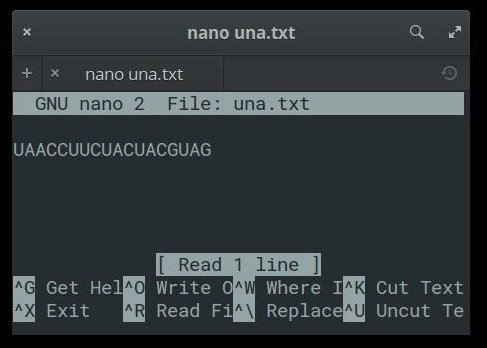
\includegraphics[width=54mm]{imgs/Labo2/INuna.jpeg}}
\subfigure[Traducción de la cadena.]{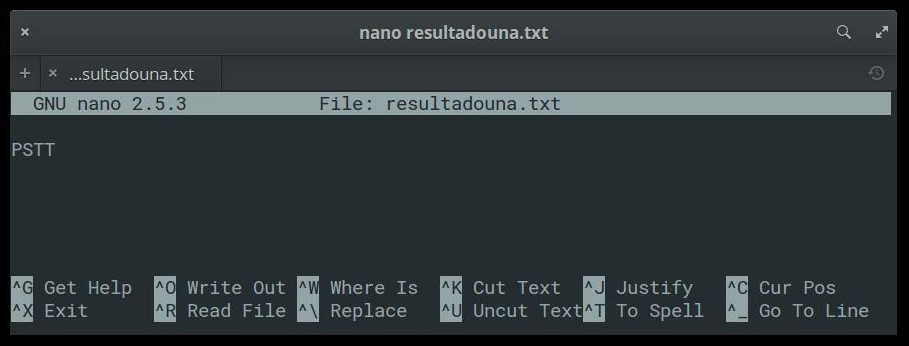
\includegraphics[width=101.5mm]{imgs/Labo2/OUTuna.jpeg}}
\caption{Traducción de una única línea.} \label{fig:trans1}
\end{figure}

Cuando al programa se le indica una ruta de un archivo con varias líneas como el que se observa en la imagen izquierda de la Figura \ref{fig:trans2}, este se ejecuta de igual manera, y escribe un archivo con la traducción correspondiente como se observa en la imagen de la derecha.

\begin{figure}[htbp]
\centering
\subfigure[Varias cadenas de codones.]{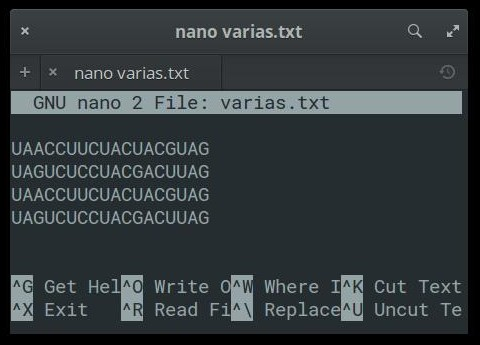
\includegraphics[width=54mm]{imgs/Labo2/INvarias.jpeg}}
\subfigure[Traducción de las cadenas.]{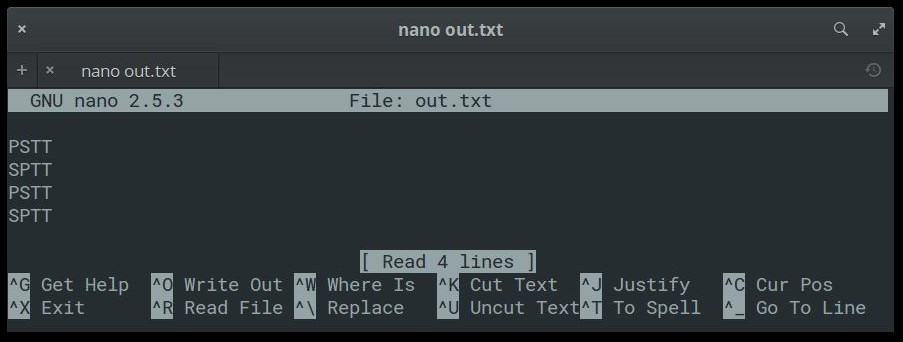
\includegraphics[width=102mm]{imgs/Labo2/OUTvarias.jpeg}}
\caption{Traducción de varias cadenas de codones.} \label{fig:trans2}
\end{figure}

\section{Conclusiones}
El objetivo principal del laboratorio se cumplió satisfactoriamente. Se logró familiarizarse con los comandos de C++ y el paradigma de programación orientada a objetos. También es importante notar el uso del concepto de reserva de memoria dinámica, así como su debida liberación después de su uso. Además se practicó la correcta documentación del código utilizando \texttt{Doxygen}, y la compilación mediante un \texttt{makefile}. 


%%%%%%%%%%%%%%%%%%
%--> LABORATORIO 3
%%%%%%%%%%%%%%%%%%
%%%%%%%%%%%%%%%%%%%%%%%%%%%%%%%%%%%%%%%%%%%%%%%%%%%%%%%%%%%%%%%%%%%%%%%%%%%%%%%%%%%%%%%%%%%%%%%%%%%%
\newpage
\section{Introducción}
%%%%%%%%%%%%%%%%%%%%%%%%%%%%%%%%%%%%%%%%%%%%%%%%%%%%%%%%%%%%%%%%%%%%%%%%%%%%%%%%%%%%%%%%%%%%%%%%%%%

Se define herencia como el proceso mediante el cual una clase adquiere las propiedades (atributos) y comportamientos (métodos) de otra clase. 

En programación orientada a objetos comprender los conceptos de herencia, polimorfismo, funciones virtuales y sobrecarga es de vital importancia para lograr aplicar el concepto de clases a la resolución de diferentes tipos de problemas en las que usar estos conceptos nos ayuda a modelar la solución de una manera más eficiente y adecuada. 

%%%%%%%%%%%%%%%%%%%%%%%%%%%%%%%%%%%%%%%%%%%%%%%%%%%%%%%%%%%%%%%%%%%%%%%%%%%%%%%%%%%%%%%%%%%%%%%%%%%
\subsection{Objetivos}
\begin{enumerate}
\item Repasar y utilizar los conceptos de herencia, polimorfismo y sobrecarga. 
\item Practicar la sobrecarga de operadores para simplificar algunas operaciones.
\item Realizar un diagrama UML que permita visualizar la relación entre clases. 
\end{enumerate}
%%%%%%%%%%%%%%%%%%%%%%%%%%%%%%%%%%%%%%%%%%%%%%%%%%%%%%%%%%%%%%%%%%%%%%%%%%%%%%%%%%%%%%%%%%%%%%%%%%%
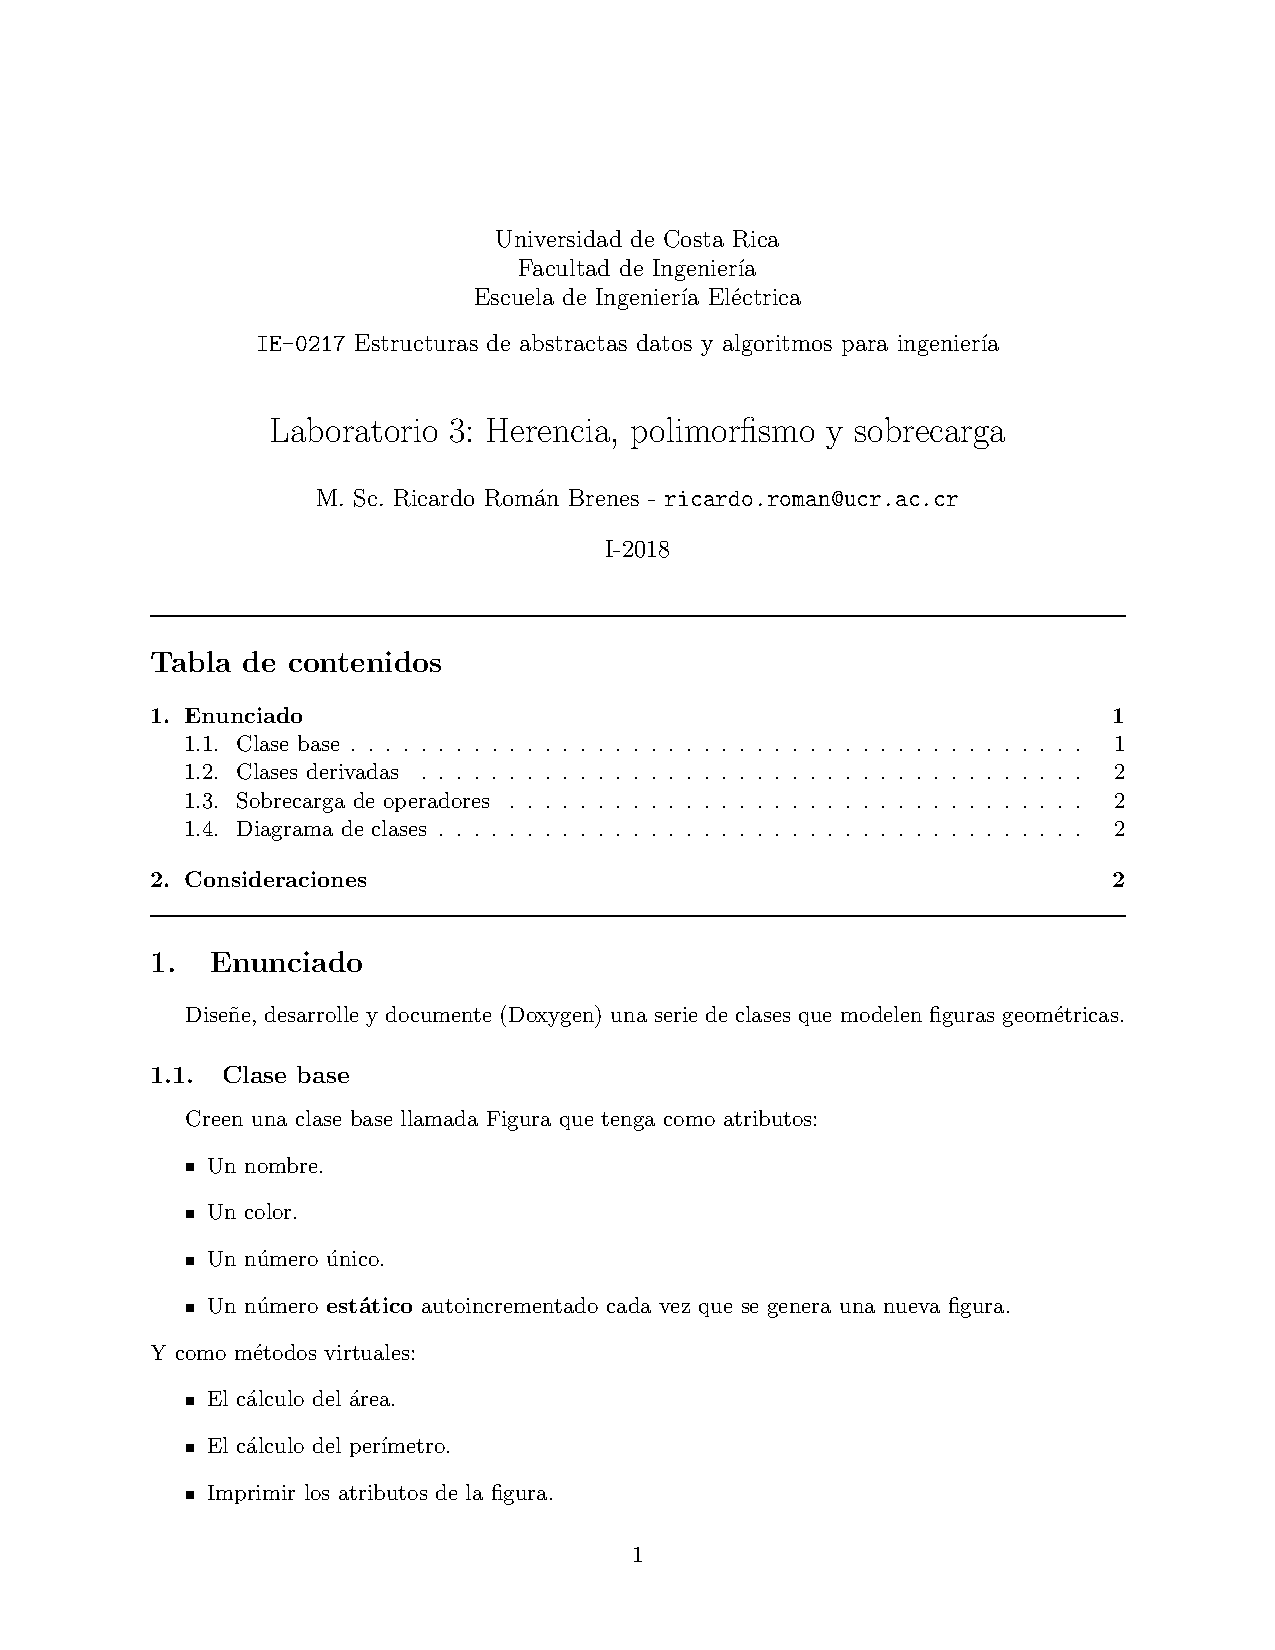
\includepdf[pages=1,pagecommand=\section{Enunciado}]{enunciados/enun3}
\includepdf[pages=2,pagecommand={}]{enunciados/enun3}
%%%%%%%%%%%%%%%%%%%%%%%%%%%%%%%%%%%%%%%%%%%%%%%%%%%%%%%%%%%%%%%%%%%%%%%%%%%%%%%%%%%%%%%%%%%%%%%%%%%

%%%%%%%%%%%%%%%%%%%%%%%%%%%%%%%%%%%%%%%%%%%%%%%%%%%%%%%%%%%%%%%%%%%%%%%%%%%%%%%%%%%%%%%%%%%%%%%%%%%
\section{Solución}
%\begin{minted}[linenos,autogobble,bgcolor=bg,breaklines,fontsize=\footnotesize ]{c++}

%\end{minted}
%%%%%%%%%%%%%%%%%%%%%%%%%%%%%%%%%%%%%%%%%%%%%%%%%%%%%%%%%%%%%%%%%%%%%%%%%%%%%%%%%%%%%%%%%%%%%%%%%%%
\subsection{Clase base: \texttt{Figure()}}
La clase \texttt{Figure()} es la clase base del programa, de donde las demás clases heredan. En el \textit{header} \texttt{Figure.h} se definen los métodos y atributos de la clase. En la sección pública se colocan las definiciones de los métodos constructor, destructor, así como los métodos virtuales para calcular el área, el perímetro, y la función encargada de imprimir los datos de la clase. Se declaran los atributos como protegidos, en estos se incluye el nombre, el color, un número único para el objeto, y un número estático que se incrementa cada vez que se genera una figura, para esto se implementa un método más.

\begin{minted}[linenos,autogobble,bgcolor=bg,breaklines,fontsize=\footnotesize ]{c++}
#include <string>
#include <iostream>
using namespace std;
#ifndef FIGURE_H
#define FIGURE_H

///@class Figure
class Figure {
  public:
    Figure();
    ~Figure();
    virtual double area() = 0 ; 
    virtual double perimetro() = 0; 
    virtual void imprimir() = 0;
  protected:
    int getNumAutoInc();
    string nombre;
    string color;
    int numUnico;
    static int numAutoInc; 
  private:
};
#endif
\end{minted}

\subsection{Clase derivada: \texttt{Rectangle()}}

La clase \texttt{Rectangle()} hereda de la clase base; como se observa a la hora de declararlo mediante la línea \texttt{class Rectangle : public Figure}. En el archivo \texttt{Rectangle.h} se observan los métodos que contiene esta clase. Para los cálculos respectivos a un rectángulo, se declaran dos variables protegidas de tipo \texttt{double} para almacenar el largo y el ancho de la figura.
\begin{minted}[linenos,autogobble,bgcolor=bg,breaklines,fontsize=\footnotesize ]{c++}
#include <string>
#include <iostream>
#include "../include/Figure.h"
using namespace std;
#ifndef RECTANGLE_H
#define RECTANGLE_H

///@class Rectangle
class Rectangle : public Figure {
  public:
    Rectangle();
    Rectangle(string nombre, string color, int numUnico, double largo, double ancho);
    Rectangle(const Rectangle& r);
    ~Rectangle();
    double area();
    double perimetro();
    void imprimir();
    void operator~();
    void operator!();
    void operator=(const Rectangle& r);
  protected:
    double largo;
    double ancho;
  private:
};
#endif
\end{minted}

\subsubsection{Métodos de \texttt{Rectangle()}}
\begin{itemize}
\item \textbf{Constructor vacío:}

	Cuando se crea un objeto de tipo \texttt{Rectangle} sin pasarle ningún argumento, se utiliza este constructor. Aquí se le solicita al usuario que ingrese los datos necesarios para crear el objeto con sus atributos bien definidos. Se solicita el nombre, el color, el número único y las medidas de los lado, todo lo anterior se guarda en las variables de los atributos respectivos utilizando el operador \texttt{this->}.
    \begin{minted}[linenos,autogobble,bgcolor=bg,breaklines,fontsize=\footnotesize ]{c++}
Rectangle::Rectangle(){
  cout << endl <<"Ingrese el nombre del rectangulo:  ";
  cin >> this->nombre;
  cout << endl << "Ingrese el color del rectangulo:  ";
  cin >> this->color;
  cout << endl << "Ingrese un numero unico para identificar el rectangulo:  ";
  cin >> this->numUnico;
  cout << endl << "Ingrese la medidad del lado largo del rectangulo:  ";
  cin >> this->largo;
  cout << endl << "Ingrese la medidad del ancho del rectangulo:  ";
  cin >> this->ancho;
}   
    \end{minted}
    
\item \textbf{Constructor con parámetros:}

	El constructor con parámetros se utiliza cuando se crea un objeto y se le pasan los atributos como argumentos al método.
	\begin{minted}[linenos,autogobble,bgcolor=bg,breaklines,fontsize=\footnotesize ]{c++}
Rectangle::Rectangle(string nombre, string color, int numUnico, double largo, double ancho) {
  this->nombre = nombre;
  this->color = color;
  this->numUnico = numUnico;
  this->largo = largo;
  this->ancho = ancho;
}
   \end{minted}

\item \textbf{Constructor por copia:}

Para crear un objeto inicializándolo con otro ya existente. Se pasa una referencia al objeto existente, y se copian sus atributos en el nuevo objeto.

\begin{minted}[linenos,autogobble,bgcolor=bg,breaklines,fontsize=\footnotesize ]{c++}
Rectangle::Rectangle(const Rectangle &copyRectangle){
  this->nombre    = copyRectangle.nombre;
  this->color     = copyRectangle.color;
  this->numUnico  = copyRectangle.numUnico;
  this->largo     = copyRectangle.largo;
  this->ancho     = copyRectangle.ancho;
}
\end{minted}

\item \textbf{Área y perímetro:}

	Los dos métodos para calcular el área y el perímetro simplemente en el \texttt{return} realizan la operación necesaria para obtener el resultado. Para obtener las medidas de los lados se utilizan los atributos utilizando el puntero \texttt{this->}. Por el tipo de cálculo a realizar, las funciones devuelven el resultado tipo \texttt{double}.
    
	\begin{minted}[linenos,autogobble,bgcolor=bg,breaklines,fontsize=\footnotesize ]{c++}
double Rectangle::area(){
  return (this->largo*this->ancho);
}
\end{minted}

	\begin{minted}[linenos,autogobble,bgcolor=bg,breaklines,fontsize=\footnotesize ]{c++}
double Rectangle::perimetro(){
  return ((2*(this->largo))+(2*(this->ancho)));
}
\end{minted}

\item \textbf{Método imprimir:}

	Imprime todos los datos del objeto.
    	\begin{minted}[linenos,autogobble,bgcolor=bg,breaklines,fontsize=\footnotesize ]{c++}
void Rectangle::imprimir() {
  cout << "Nombre: " << this->nombre << endl;
  cout << "Color: " << this->color << endl;
  cout << "Número Único: " << this->numUnico << endl;
  cout << "Largo: " << this->largo << endl;
  cout << "Ancho: " << this->ancho << endl;
  cout << "Número Autoincrementado: " << this->numAutoInc << endl;
}
\end{minted}

\item \textbf{Sobrecarga de operadores}\\
Se implementa la sobrecarga de los operadores \texttt{!, \~} y \texttt{=}. El operador \texttt{!} se utiliza para calcular el área y el perímetro; \texttt{\~} se utiliza para imprimir los datos del objeto, y el operador \texttt{=} se utiliza para igualar o copiar un objeto en otro.

\begin{minted}[linenos,autogobble,bgcolor=bg,breaklines,fontsize=\footnotesize ]{c++}
void Rectangle::operator~(){
  imprimir();
}
void Rectangle::operator!(){
  cout << "Area: " << area() << endl;
  cout << "Perimetro: " << perimetro() << endl;
}
void Rectangle::operator=(const Rectangle& r)
{
  this->nombre    = r.nombre;
  this->color     = r.color;
  this->numUnico  = r.numUnico;
  this->largo     = r.largo;
  this->ancho     = r.ancho;
}
\end{minted}


\end{itemize}



\subsection{Clase derivada: \texttt{Triangle()}}

\begin{minted}[linenos,autogobble,bgcolor=bg,breaklines,fontsize=\footnotesize ]{c++}
#include <string>
#include <iostream>
#include "../include/Figure.h"
#ifndef TRIANGLE_H
#define TRIANGLE_H

class Triangle : public Figure
{
  public:
    Triangle();
    Triangle(string n, string c, int num, double l1, double l2, double l3);
    Triangle(const Triangle& r);
    ~Triangle();
    double area();
    double perimetro();
    void imprimir();
    void operator~();
    void operator!();
    void operator=(const Triangle& t);
  private:
	  double lado1;
	  double lado2;
	  double lado3;
	  string tipo;	//tipo de triangulo
	  void initIDs();	//para pedir valores de atributos al usuario
  	void initLados(); //para pedir valores de los lados al usuario
  	bool desigualdad(double a, double b, double c); //teorema de la desigualdad para ver si con lados ingresados se puede formar un triangulo
  	bool verifLados(double l1, double l2, double l3);
  	void verifTipo(double l1, double l2, double l3);
  };

#endif

\end{minted}

\subsubsection{Métodos de \texttt{Triangle()}}

\begin{itemize}
\item \textbf{Constructor vacío:}\\
Si se crea una instancia de \texttt{Triangle} utilizando el constructor vacío, se llamará a los métodos que se encargan de inicializar los atributos correspondientes. De esta manera, no se permite que existan objetos sin alguno de los atributos asignado.
\begin{minted}[linenos,autogobble,bgcolor=bg,breaklines,fontsize=\footnotesize ]{c++}
Triangle::Triangle(){
	initIDs();
	initLados();
	verifTipo(this->lado1,this->lado2,this->lado3);
}
\end{minted}

\item \textbf{Constructor con parámetros:}\\
Se puede crear un objeto \texttt{Triangle} pasándole los atributos en el constructor, en un orden específico. En este caso, se debe llamar a un método que verifica si los lados con los que se desea construir este objeto son válidos (más adelante se explica de qué se trata esto).
\begin{minted}[linenos,autogobble,bgcolor=bg,breaklines,fontsize=\footnotesize ]{c++}
Triangle::Triangle(string n, string c, int num, double l1, double l2, double l3){
	if (verifLados(l1,l2,l3) == false){
		initLados();
	}
	else {
		this->lado1 = l1;
		this->lado2 = l2;
		this->lado3 = l3;
	}
	this->nombre = n;
	this->color = c;
	this->numUnico = num;
	verifTipo(this->lado1,this->lado2,this->lado3);
}
\end{minted}

\item \textbf{Constructor por copia:}\\
Para crear un objeto inicializándolo con otro ya existente. Se pasa una referencia al objeto existente. 

\begin{minted}[linenos,autogobble,bgcolor=bg,breaklines,fontsize=\footnotesize ]{c++}
Triangle::Triangle(const Triangle &copy){
  this->nombre    = copy.nombre;
  this->color     = copy.color;
  this->numUnico  = copy.numUnico;
  this->lado1     = copy.lado1;
  this->lado2     = copy.lado2;
  this->lado3     = copy.lado3;
  this->tipo      = copy.tipo;
}
\end{minted}


\item \textbf{Inicializador de identificadores (\texttt{initIDs()})}\\
Así se denominó al método que solicita al usuario los valores de los atributos \texttt{nombre}, \texttt{color} y \texttt{numUnico}, para asignárselos al objeto creado. No se hace verificación de tipos. 

\begin{minted}[linenos,autogobble,bgcolor=bg,breaklines,fontsize=\footnotesize ]{c++}
void Triangle::initIDs(){
	string n, c;
	int num;
	cout << endl << "Ingrese el nombre del triangulo:  ";
	cin >> n;
	cout << endl << "Ingrese el color del triangulo:  ";
	cin >> c;
	cout << endl << "Ingrese un numero unico para identificar el triangulo: ";
	cin >> num;
	this->nombre = n;
	this->color = c;
	this->numUnico = num;
}
\end{minted}

\item \textbf{Método \texttt{initLados()}}\\
Solicita al usuario los valores de los lados, de tipo \texttt{double}. Antes de asignarle estos valores al objeto creado, utiliza el método \texttt{verifLados()} para determinar si son valores válidos. El ciclo \texttt{do ... while} permite ejecutar la solicitud al usuario, y luego verificar si se cumple la condición; de no ser así, la solicitud se vuelve a realizar.

\begin{minted}[linenos,autogobble,bgcolor=bg,breaklines,fontsize=\footnotesize ]{c++}
void Triangle::initLados(){
	double l1, l2, l3;
	do {
		cout << endl <<"Ingrese el primer lado: ";
		cin >> l1;
		cout << endl << "Ingrese el segundo lado:  ";
		cin >> l2;
		cout << endl << "Ingrese el tercer lado:  ";
		cin >> l3;
	} while (verifLados(l1,l2,l3)==false);
	this->lado1 = l1;
	this->lado2 = l2;
	this->lado3 = l3;
}
\end{minted}

\item \textbf{Método \texttt{verifLados()}}\\
Este método verifica si los valores que se quiere asignar a los lados del triángulo creado, son valores válidos; esto es, si cumplen el teorema de la desigualdad triangular. Este teorema establece que los lados l1, l2 y l3 forman un triángulo si la suma de cualesquiera dos de ellos es mayor al lado restante. Este teorema se implementa aquí con otro método llamado \texttt{desigualdad()}, que retorna un valor booleano. Se indica en un mensaje si los lados ingresados son válidos.

\begin{minted}[linenos,autogobble,bgcolor=bg,breaklines,fontsize=\footnotesize ]{c++}
bool Triangle::verifLados(double l1, double l2, double l3){
	if (desigualdad(l1,l2,l3) == true){
		cout << endl << "Lados válidos" << endl << endl;
		return true;
	}
	else{
		cout << endl<< "Los lados ingresados (" << l1 << "," << l2 << "," << l3 << ") no pueden formar un triángulo. Ingrese lados válidos." << endl;
		return false;
	}
}

bool Triangle::desigualdad(double a, double b, double c){
	if ((a<b+c) && (b<a+c) && (c<a+b)){
		return true;
	}
	else {
		return false;
	}
}
\end{minted}

\item \textbf{Método \texttt{verifTipo()}}\\
Evalúa los lados del triángulo para determinar si este es ``equilátero'', ``isósceles'' o ``escaleno'', y asigna el valor resultante al atributo \texttt{tipo}.

\begin{minted}[linenos,autogobble,bgcolor=bg,breaklines,fontsize=\footnotesize ]{c++}
void Triangle::verifTipo(double l1, double l2, double l3){
	if (l1 == l2 && l2 == l3){
		this->tipo="equilatero";
	}
	else if ((l1==l2)||(l1==l3)||(l2==l3)){
		this->tipo="isosceles";
	}
	else {
		this->tipo="escaleno";
	}
}
\end{minted}

\item \textbf{Métodos \texttt{perimetro()} y \texttt{area()}}\\
El método \texttt{perimetro()} devuelve la suma de los lados, mientras que \texttt{area()} calcula el área a partir de los lados utilizando la fórmula de Herón:

\begin{equation}
A = \sqrt[]{s(s-a)(s-b)(s-c)}
\end{equation}

Donde $s$ es el valor del semiperímetro, es decir, la mitad del valor retornado por \texttt{perimetro()}. Para este cálculo se utilizó la función \texttt{sqrt()} de la biblioteca \texttt{math.c}. 

\begin{minted}[linenos,autogobble,bgcolor=bg,breaklines,fontsize=\footnotesize ]{c++}
double Triangle::perimetro(){
	return (this->lado1+this->lado2+this->lado3);
}

double Triangle::area(){
	double a = this->lado1, b = this->lado2, c = this->lado3;
	double semip = perimetro()/2;
	double heron = (semip*(semip-a)*(semip-b)*(semip-c));
	return sqrt(heron);
}
\end{minted}

\item \textbf{Método \texttt{imprimir()}}\\
Imprime en pantalla todos los atributos del objeto.

\begin{minted}[linenos,autogobble,bgcolor=bg,breaklines,fontsize=\footnotesize ]{c++}
void Triangle::imprimir() {
	cout << "Nombre: " << this->nombre << endl;
	cout << "Color: " << this->color << endl;
	cout << "Número Único: " << this->numUnico << endl;
	cout << "Tipo: " << this->tipo << endl;
	cout << "Lado 1: " << this->lado1 << endl;
	cout << "Lado 2: " << this->lado2 << endl;
	cout << "Lado 3: " << this->lado3 << endl;
	cout << "Número Autoincrementado: " << this->numAutoInc << endl;
}
\end{minted}

\item \textbf{Sobrecarga de operadores}\\
Se implementa la sobrecarga de los operadores \texttt{!, \~} y \texttt{=}.

\begin{minted}[linenos,autogobble,bgcolor=bg,breaklines,fontsize=\footnotesize ]{c++}
void Triangle::operator~(){
  imprimir();
}

void Triangle::operator!(){
  cout << "Area: " << area() << endl;
  cout << "Perimetro: " << perimetro() << endl;
}

void Triangle::operator=(const Triangle& t){
  this->nombre		= t.nombre;
  this->color		= t.color;
  this->numUnico	= t.numUnico;
  this->lado1		= t.lado1;
  this->lado2		= t.lado2;
  this->lado3		= t.lado3;
  this->tipo		= t.tipo;
}
\end{minted}

\end{itemize}

\subsection{Clase derivada: \texttt{Circle()}}
Como se observa a la hora de declarar la clase mediante la línea \texttt{class Circle : public Figure}, la clase \texttt{Circle()} hereda de la clase base. En el archivo \texttt{Circle.h} se observan los métodos que contiene esta clase. Para los cálculos respectivos del círculo, se declara una variable privada de tipo \texttt{double} para almacenar el radio de la figura.

\subsubsection{Métodos de \texttt{Circle()}}
\begin{minted}[linenos,autogobble,bgcolor=bg,breaklines,fontsize=\footnotesize ]{c++}
#include <string>
#include <iostream>
#include "../include/Figure.h"
using namespace std;
#ifndef CIRCLE_H
#define CIRCLE_H

class Circle : public Figure
{
  public:
    Circle();
    Circle(string nombre, string color, int numUnico, double radio);
    // Circle(const Circle& r);
    ~Circle();
    double area();
    double perimetro();
    void imprimir();
    void operator~();
    void operator!();
    void operator=(const Circle& r);
    //void operator=(Circle r);
  protected:
  private:
    double radio;
};
#endif
\end{minted}

\begin{itemize}
\item \textbf{Métodos constructores:}

	Para crear un nuevo objeto de tipo \texttt{Circle} se implementaron dos constructores, uno de ellos vacío que conforme se ejecuta se le piden al usuario los valores de los atributos del objeto. El otro constructor recibe como argumentos los parámetros mencionados. También se implementa el constructor por copia.
    
\begin{minted}[linenos,autogobble,bgcolor=bg,breaklines,fontsize=\footnotesize ]{c++}
Circle::Circle()
{
  cout << endl <<"Ingrese el nombre del círculo: ";
  cin >> this->nombre;
  cout << endl << "Ingrese el color del círculo: ";
  cin >> this->color;
  cout << endl << "Ingrese un número único para identificar el círculo: ";
  cin >> this->numUnico;
  cout << endl << "Ingrese la medida del radio del círculo: ";
  cin >> this->radio;
}
Circle::Circle(string nombre, string color, int numUnico, double radio)
{
  this->nombre    = nombre;
  this->color     = color;
  this->numUnico  = numUnico;
  this->radio     = radio;
}
\end{minted}

\item \textbf{Área y perímetro:}

	Los dos métodos para calcular el área y el perímetro simplemente en el \texttt{return} realizan la operación necesaria para obtener el resultado. Para obtener las medidas de los lados se utilizan los atributos utilizando el puntero \texttt{this->}. Por el tipo de cálculo a realizar, las funciones devuelven el resultado tipo \texttt{double}. Es importante destacar que para el cálculo del área se debe multiplicar por $\pi$, por lo que se define al inicio del archivo utilizando \texttt{\#define}.
    
	\begin{minted}[linenos,autogobble,bgcolor=bg,breaklines,fontsize=\footnotesize ]{c++}
    #define PI 3.14159265358979323846
\end{minted}
    
	\begin{minted}[linenos,autogobble,bgcolor=bg,breaklines,fontsize=\footnotesize ]{c++}
double Circle::area()
{
  return (PI*this->radio*this->radio);
}
\end{minted}

	\begin{minted}[linenos,autogobble,bgcolor=bg,breaklines,fontsize=\footnotesize ]{c++}
double Circle::perimetro()
{
  return (2.0*this->radio*PI);
}
\end{minted}

\item \textbf{Método imprimir y sobrecarga de los operadores \texttt{=} , \texttt{!} , \texttt{\~} :}

Al igual que en las clases anteriores se implementa un método para imprimir los datos del objetos. Además los operadores se definen para imprimir los datos del objeto, para calcular el área y el perímetro, y para igual o crear una copia de un objeto.

\begin{minted}[linenos,autogobble,bgcolor=bg,breaklines,fontsize=\footnotesize ]{c++}
void Circle::imprimir()
{
  cout << "Nombre: " << this->nombre << endl;
  cout << "Color: " << this->color << endl;
  cout << "Número Único: " << this->numUnico << endl;
  cout << "Radio: " << this->radio << endl;
  cout << "Número Autoincrementado: " << this->numAutoInc << endl;
}
\end{minted}
\begin{minted}[linenos,autogobble,bgcolor=bg,breaklines,fontsize=\footnotesize ]{c++}
void Circle::operator~()
{
  imprimir();
}
void Circle::operator!()
{
  cout << "Area: " << area() << endl;
  cout << "Perimetro: " << perimetro() << endl;
}
void Circle::operator=(const Circle& r)
{
  this->nombre    = r.nombre;
  this->color     = r.color;
  this->numUnico  = r.numUnico;
  this->radio     = r.radio;
}
\end{minted}


\end{itemize}

\subsection{Diagrama de clases.}
En la Figura \ref{fig:dia} se puede observar el diagrama de las clases implementadas. Las clases derivadas \texttt{Rectangle}, \texttt{Triangle} y \texttt{Circle} heredan de la clase base \texttt{Figure}, como se observa en la Figura \ref{fig:dia} mediante una flecha. Además se pueden observar los atributos y métodos que conforman cada una de ellas.
\begin{figure}[H]
  \centering
    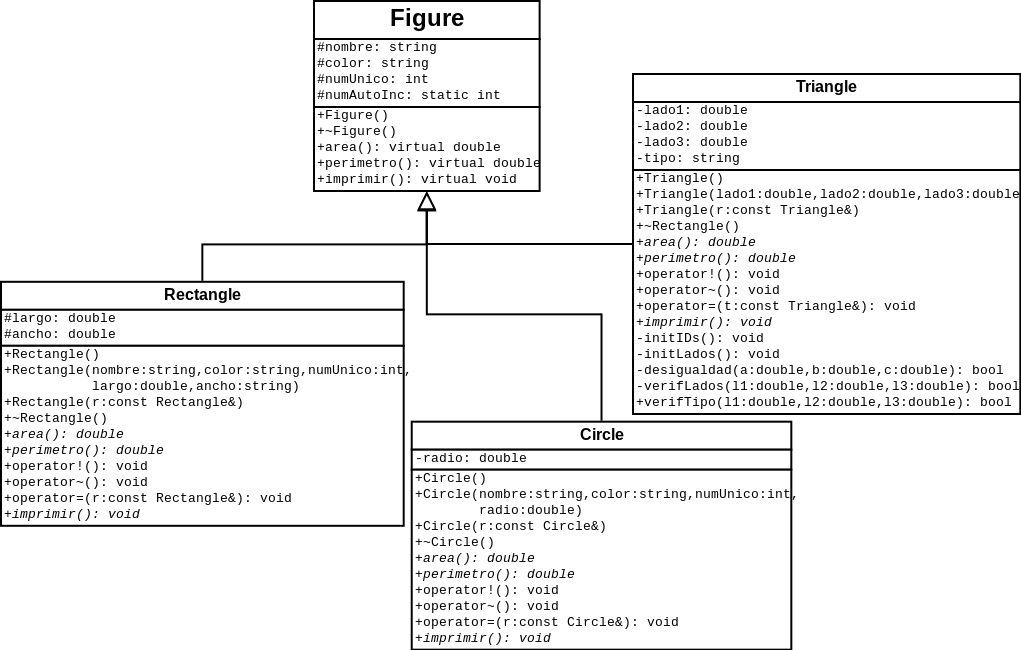
\includegraphics[width=\textwidth]{imgs/Labo3/Diagram1.png}
  \caption{Diagrama de clases}
  \label{fig:dia}
\end{figure}

%%%%%%%%%%%%%%%%%%%%%%%%%%%%%%%%%%%%%%%%%%%%%%%%%%%%%%%%%%%%%%%%%%%%%%%%%%%%%%%%%%%%%%%%%%%%%%%%%%%
\newpage
\section{Resultados}
%%%%%%%%%%%%%%%%%%%%%%%%%%%%%%%%%%%%%%%%%%%%%%%%%%%%%%%%%%%%%%%%%%%%%%%%%%%%%%%%%%%%%%%%%%%%%%%%%%%
Para observar los resultados de la implementación de las clases descritas, se creó un programa \texttt{main} en el que se crean algunos objetos. 

Para comprobar la funcionalidad de la clase \texttt{Circle}, se crea un objeto con el constructor vacío, lo cual causa que el programa solicite al usuario que ingrese los valores de los atributos:

\begin{minted}[linenos,autogobble,bgcolor=bg,breaklines,fontsize=\footnotesize ]{c++}
Circle circulo1 = Circle();
\end{minted}

Luego de esto se imprime los datos de información de la figura, área y perímetro, haciendo uso de la sobrecarga de los operadores $!$ y $\sim$. Posteriormente, se crea otra clase, pero esta vez pasándole los parámetros de los atributos a través del constructor:

\begin{minted}[linenos,autogobble,bgcolor=bg,breaklines,fontsize=\footnotesize ]{c++}
Circle circulo2("Circulo #2","Rojo",3,3.4);
\end{minted}

Por último, se comprueba el resultados de sobrecargar el operador = al igualar el primer circulo creado con el segundo. Los resultados de estas pruebas se pueden ver en la Figura \ref{fig:CIRC}.

\begin{figure}[H]
\centering
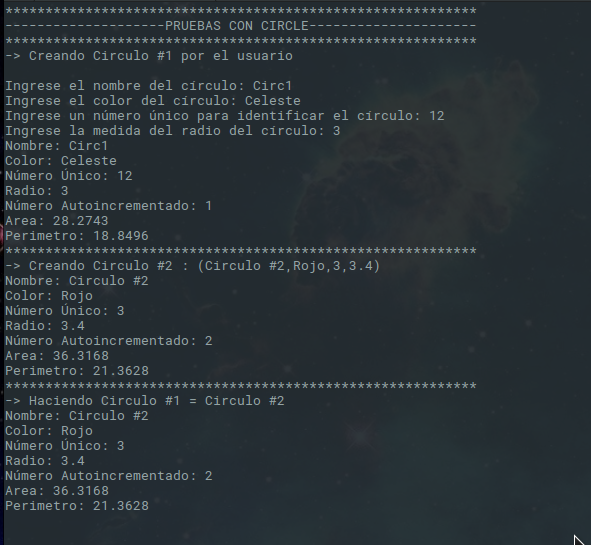
\includegraphics[width=.7\textwidth]{imgs/Labo3/CIRC}
\caption{Resultado de la implementación de la clase \texttt{Circle}}
\label{fig:CIRC}
\end{figure}

Una prueba similar se realizó para comprobar las funcionalidad de la clase \texttt{Rectangle} y los resultados se pueden ver en la Figura \ref{fig:RECT}.

\begin{figure}[H]
\centering
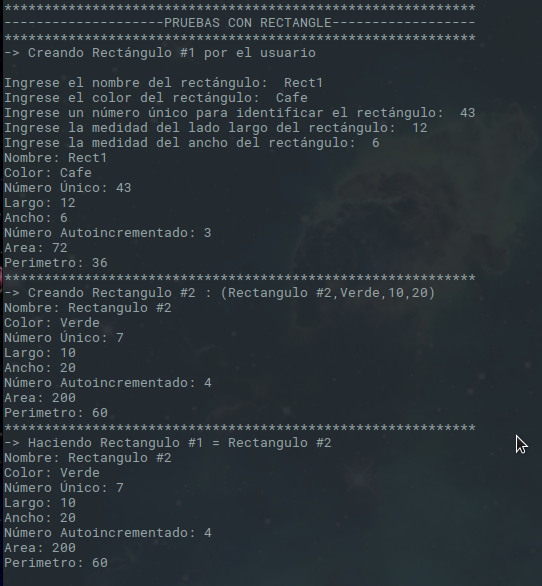
\includegraphics[width=.7\textwidth]{imgs/Labo3/RECT}
\caption{Resultado de la implementación de la clase \texttt{Rectangle}}
\label{fig:RECT}
\end{figure}

En la clase \texttt{Triangle}, también se hace una verificación para comprobar que los datos ingresados son válidos. En la Figura \ref{fig:TRI1}, se logra observar que si se ingresa lados que no cumplen para ser un triángulo, se solicita al usuario volver a ingresar datos.

\begin{figure}[H]
\centering
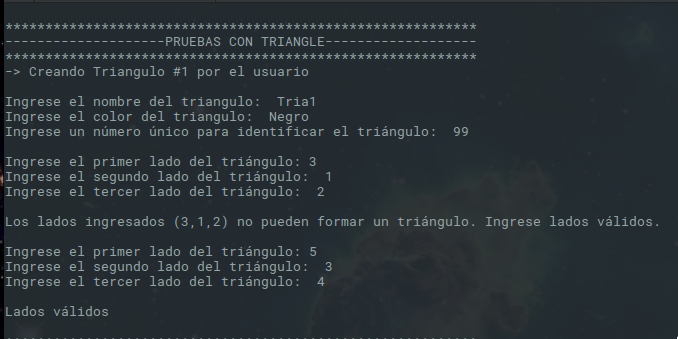
\includegraphics[width=.7\textwidth]{imgs/Labo3/TRI1}
\caption{Resultado de la implementación de la clase \texttt{Triangle}}
\label{fig:TRI1}
\end{figure}

Por último, se realizó la misma que para el círculo y rectángulo y los resultados se pueden ver en la Figura \ref{fig:TRI2}.

\begin{figure}[H]
\centering
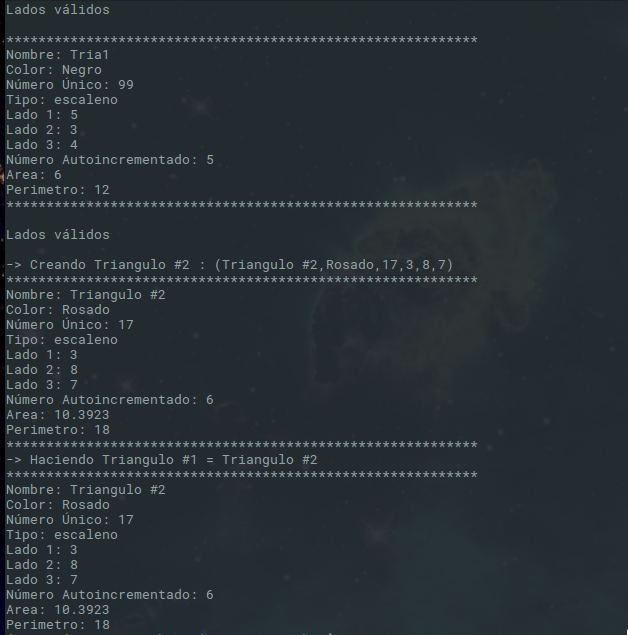
\includegraphics[width=.7\textwidth]{imgs/Labo3/TRI2}
\caption{Resultado de la implementación de la clase \texttt{Triangle}}
\label{fig:TRI2}
\end{figure}

Para correr toda la prueba es necesario ejecutar en la terminal el siguiente comando:

\begin{minted}[linenos,autogobble,bgcolor=bg,breaklines,fontsize=\footnotesize ]{bash}
make test
\end{minted}

%%%%%%%%%%%%%%%%%%%%%%%%%%%%%%%%%%%%%%%%%%%%%%%%%%%%%%%%%%%%%%%%%%%%%%%%%%%%%%%%%%%%%%%%%%%%%%%%%%%
\newpage
\section{Conclusiones}
 Como conclusiones se tiene que:
 
\begin{itemize}
\item A partir de una clase base se logra crear clases derivadas que contienen métodos y atributos heredados de la clase base, con esto se logra comprender el concepto de herencia en programación orientada a objetos.
\item Se implementó cuatro clases, con las cuales se logra crear círculos, rectángulos y triángulos y calcular su respectiva área y perímetro. 
\item Se logra sobrecargar operadores para darles diferentes usos y simplificar así la notación de las operaciones con objetos.
\item Se crea un diagrama UML con ejemplifica de mejor manera la jerarquía de las cuatro clases creadas en este proyecto.
\end{itemize}
%%%%%%%%%%%%%%%%%%%%%%%%%%%%%%%%%%%%%%%%%%%%%%%%%%%%%%%%%%%%%%%%%%%%%%%%%%%%%%%%%%%%%%%%%%%%%%%%%%%


%%%%%%%%%%%%%%%%%%
%--> LABORATORIO 4
%%%%%%%%%%%%%%%%%%
%%%%%%%%%%%%%%%%%%%%%%%%%%%%%%%%%%%%%%%%%%%%%%%%%%%%%%%%%%%%%%
% --> INTRODUCCIÓN
%%%%%%%%%%%%%%%%%%%%%%%%%%%%%%%%%%%%%%%%%%%%%%%%%%%%%%%%%%%%%%
\section{Introducción}

Según \cite{R1} la programación genérica está mucho más centrada en los algoritmos que en los datos, y su postulado fundamental puede sintetizarse en una palabra: generalización. Significa que, en la medida de lo posible, los algoritmos deben ser parametrizados al máximo y expresados de la forma más independiente posible de detalles concretos, permitiendo así que puedan servir para la mayor variedad posible de tipos y estructuras de datos.

%%%%%%%%%%%%%%%%%%%%%%%%%%%%%%%%%%%%%%%%%%%%%%%%%%%%%%%%%%%%%%
% --> OBJETIVOS
%%%%%%%%%%%%%%%%%%%%%%%%%%%%%%%%%%%%%%%%%%%%%%%%%%%%%%%%%%%%%%
\subsection{Objetivos}

A continuación, se enlistan los objetivos de este laboratorio.

%%%%%%%%%%%%%%%%%%%%%%%%%%%%%%%%%%%%%%%%%%%%%%%%%%%%%%%%%%%%%%
% --> OBJETIVO GENERAL
%%%%%%%%%%%%%%%%%%%%%%%%%%%%%%%%%%%%%%%%%%%%%%%%%%%%%%%%%%%%%%
\subsubsection{Objetivo General}
\begin{itemize}
\item Diseñar una serie de clases con plantillas que permitan hacer operaciones básicas con enteros. reales, fracciones, polinomios y matrices.
\end{itemize}

%%%%%%%%%%%%%%%%%%%%%%%%%%%%%%%%%%%%%%%%%%%%%%%%%%%%%%%%%%%%%%
% --> OBJETIVOS ESPECÍFICOS
%%%%%%%%%%%%%%%%%%%%%%%%%%%%%%%%%%%%%%%%%%%%%%%%%%%%%%%%%%%%%%
\subsubsection{Objetivos Específicos}
\begin{itemize}
\item 
\item 
\item 
\end{itemize}

%%%%%%%%%%%%%%%%%%%%%%%%%%%%%%%%%%%%%%%%%%%%%%%%%%%%%%%%%%%%%%
% --> ENUNCIADO
%%%%%%%%%%%%%%%%%%%%%%%%%%%%%%%%%%%%%%%%%%%%%%%%%%%%%%%%%%%%%%
\newpage

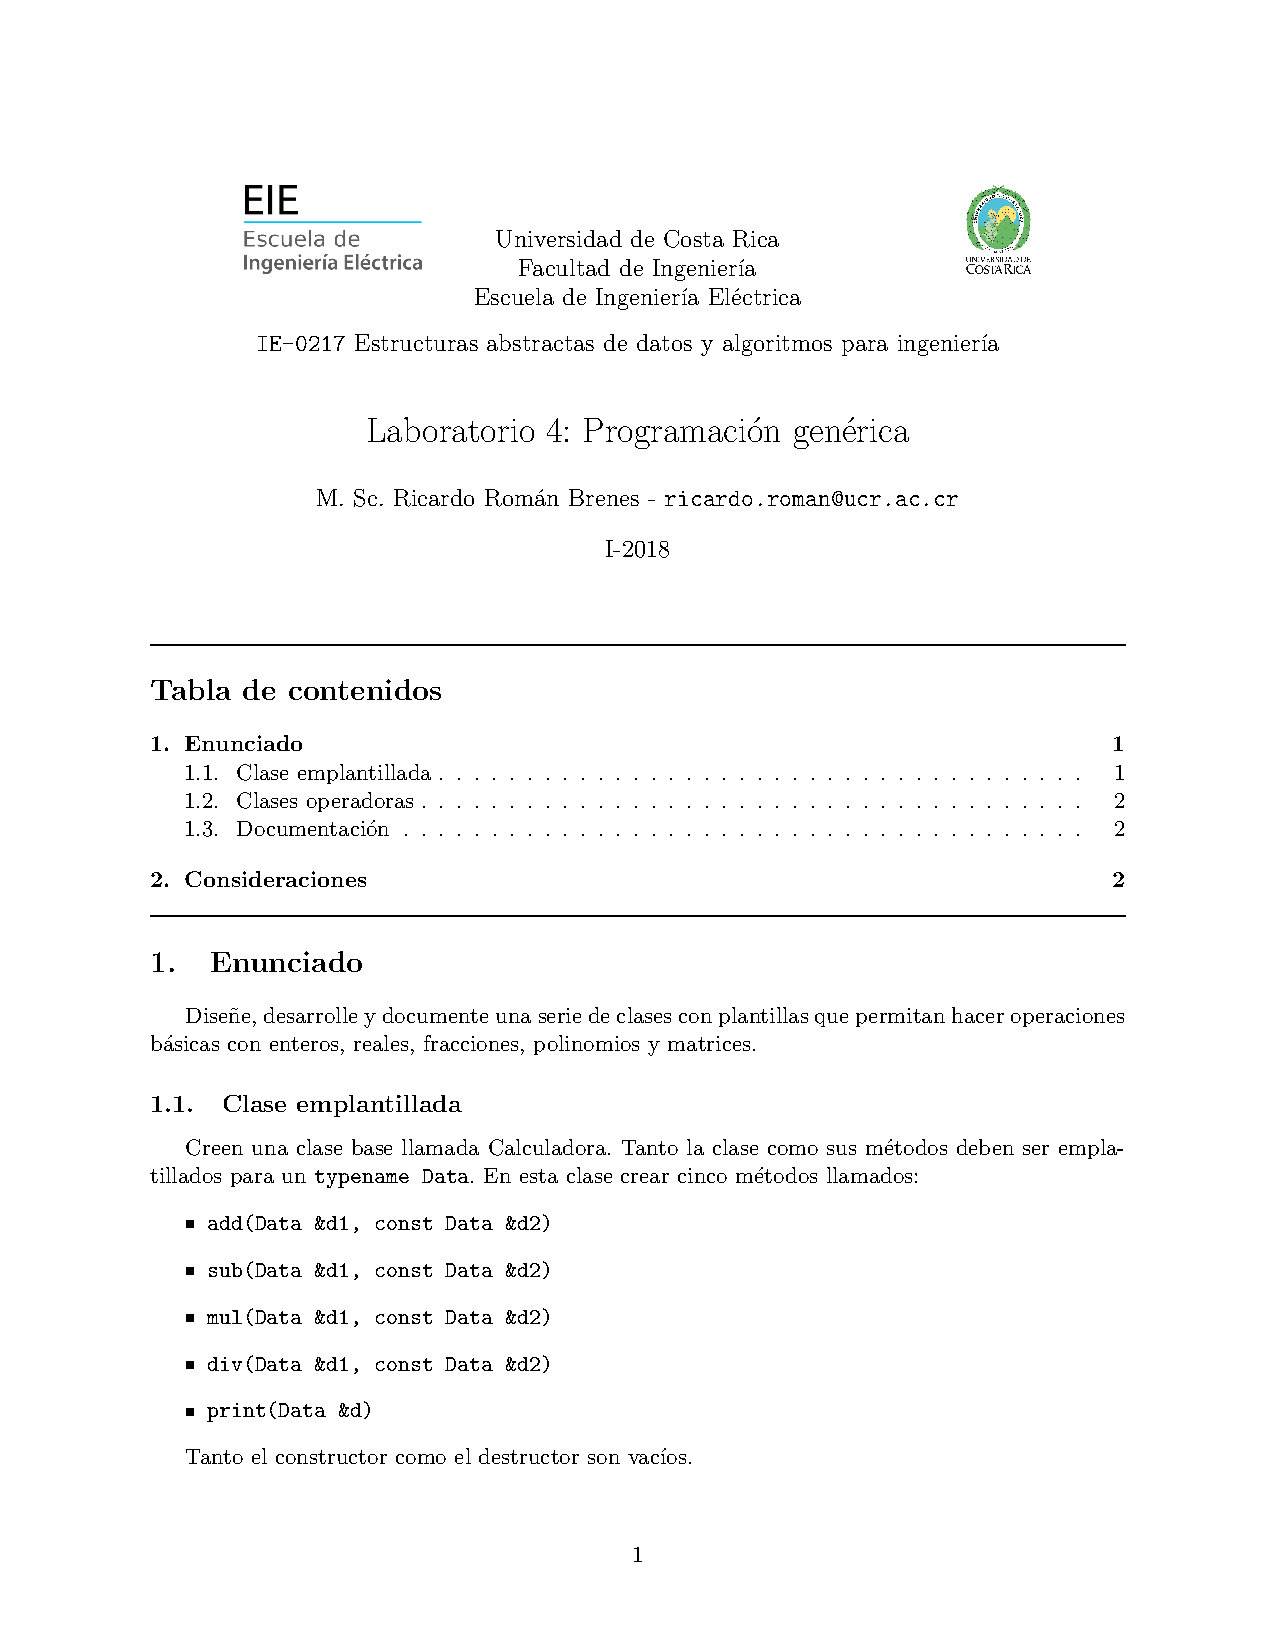
\includepdf[pages=1,pagecommand=\section{Enunciado}, scale=0.8]{enunciados/enun4} 
\includepdf[pages=2,pagecommand={},scale=0.8]{enunciados/enun4}

%%%%%%%%%%%%%%%%%%%%%%%%%%%%%%%%%%%%%%%%%%%%%%%%%%%%%%%%%%%%%%
% --> SOLUCIÓN
%%%%%%%%%%%%%%%%%%%%%%%%%%%%%%%%%%%%%%%%%%%%%%%%%%%%%%%%%%%%%%
\section{Solución}

%%%%%%%%%%%%%%%%%%%%%%%%%%%%%%%%%%%%%%%%%%%%%%%%%%%%%%%%%%%%%%
% --> CLASE POLINOMIO
%%%%%%%%%%%%%%%%%%%%%%%%%%%%%%%%%%%%%%%%%%%%%%%%%%%%%%%%%%%%%%
\subsection{Clase Polinomio}

La clase \texttt{Polynomial} realiza operaciones básicas de polinomios de grado n. En este archivo \texttt{.h} se declaran todas las funciones necesarias, así como dos variables necesarias para la ejecución, una tipo \texttt{int} para almacenar el tamaño del polinomio, es decir, la cantidad de coeficientes que posee. Y otra variable tipo \texttt{double*} para almacenar estos coeficientes, esto es un puntero que básicamente funciona como un \texttt{array}.

\begin{minted}[linenos,autogobble,bgcolor=bg,breaklines,fontsize=\footnotesize ]{c++}
class Polynomial
{
	public:
		Polynomial	(int Grado,double Coeficientes[]);
		Polynomial	(const Polynomial &l_cCopyPolynomial);
		~Polynomial	();
		Polynomial 	operator+(const Polynomial &P);
		Polynomial 	operator-(const Polynomial &P);
		Polynomial 	operator*(const Polynomial &P);
		Polynomial	operator/(const Polynomial &P);
		void 				operator~(void);
	protected:
		double* m_pCoefPolinomio;
	private:
		int m_iTamPolinomio;

};

\end{minted}

\subsubsection{Métodos de \texttt{Polynomial()}.}
\begin{itemize}
    \item \textbf{Método constructor:}
    
    El método constructor por defecto requiere de dos argumentos, uno es el grado del polinomio, y el otro es un arreglo del tipo \texttt{double} con los coeficientes que conforman el polinomio.  
\end{itemize}

%%%%%%%%%%%%%%%%%%%%%%%%%%%%%%%%%%%%%%%%%%%%%%%%%%%%%%%%%%%%%%
% --> CLASE FRACCIÓN
%%%%%%%%%%%%%%%%%%%%%%%%%%%%%%%%%%%%%%%%%%%%%%%%%%%%%%%%%%%%%%
\subsection{Clase Fracción}

\begin{minted}[linenos,autogobble,bgcolor=bg,breaklines,fontsize=\footnotesize ]{c++}
class Fraction
{
	public:
		Fraction();
		Fraction(int l_iNum, int l_iDen);
		Fraction(const Fraction &l_cCopyFraction);
		~Fraction();
		Fraction operator+(const Fraction &rhs);
		Fraction operator-(const Fraction &rhs);
		Fraction operator*(const Fraction &rhs);
		Fraction operator/(const Fraction &rhs);
		void operator~();
	protected:
	private:
		int m_iNumerador;
		int m_iDenominador;
		void checkDen();
};
\end{minted}


%%%%%%%%%%%%%%%%%%%%%%%%%%%%%%%%%%%%%%%%%%%%%%%%%%%%%%%%%%%%%%
% --> CLASE MATRIZ
%%%%%%%%%%%%%%%%%%%%%%%%%%%%%%%%%%%%%%%%%%%%%%%%%%%%%%%%%%%%%%
\subsection{Clase Matriz}

\begin{minted}[linenos,autogobble,bgcolor=bg,breaklines,fontsize=\footnotesize ]{c++}
class Matrix
{
	public:
		Matrix		(int l_iRowSize, int l_iColSize, bool l_bFlag);
		Matrix		(double* l_pMatrix, int l_iRowSize, int l_iColSize);
		Matrix		(const Matrix &l_cCopyMat);
		~Matrix		();
		Matrix 		operator+(const Matrix &rhs);
		Matrix 		operator-(const Matrix &rhs);
		Matrix 		operator*(const Matrix &rhs);
		Matrix 		operator/(const Matrix &rhs);
		int 			GetRowSize();
		int 			GetColsSize();
		double 		GetMatValue(int l_iRow, int l_iCol);
		void  		SetMatValue(int l_iRC, double l_dValue);
		void 			operator~(void);
	protected:
	private:
		double* 	m_pMatrix;
		int 			m_iRows;
		int 			m_iCols;
};
\end{minted}

%%%%%%%%%%%%%%%%%%%%%%%%%%%%%%%%%%%%%%%%%%%%%%%%%%%%%%%%%%%%%%
% --> CLASE CALCULADORA
%%%%%%%%%%%%%%%%%%%%%%%%%%%%%%%%%%%%%%%%%%%%%%%%%%%%%%%%%%%%%%
\subsection{Clase Calculadora}

\begin{minted}[linenos,autogobble,bgcolor=bg,breaklines,fontsize=\footnotesize ]{c++}
#ifndef CALCULATOR_H
#define CALCULATOR_H

#include <iostream>
#include <string>
#include <math.h>
#include "fraction.h"
#include "matrix.h"
#include "polynomial.h"

using namespace std;

template<typename Data>
class Calculator
{
	public:
		Calculator(){};
		~Calculator(){};
		Data add(Data &d1, const Data &d2) {return d1+d2;};
		Data sub(Data &d1, const Data &d2) {return d1-d2;};
		Data mul(Data &d1, const Data &d2) {return d1*d2;};
		Data div(Data &d1, const Data &d2) {return d1/d2;};
		void print(Data &d){~d;};
	protected:
	private:
};

#endif //CALCULATOR_H
\end{minted}

%%%%%%%%%%%%%%%%%%%%%%%%%%%%%%%%%%%%%%%%%%%%%%%%%%%%%%%%%%%%%%
% --> MAIN
%%%%%%%%%%%%%%%%%%%%%%%%%%%%%%%%%%%%%%%%%%%%%%%%%%%%%%%%%%%%%%
\subsection{Programa Principal}

\begin{minted}[linenos,autogobble,bgcolor=bg,breaklines,fontsize=\footnotesize ]{c++}
class Matrix
{
	public:
		Matrix		(int l_iRowSize, int l_iColSize, bool l_bFlag);
		Matrix		(double* l_pMatrix, int l_iRowSize, int l_iColSize);
		Matrix		(const Matrix &l_cCopyMat);
		~Matrix		();
		Matrix 		operator+(const Matrix &rhs);
		Matrix 		operator-(const Matrix &rhs);
		Matrix 		operator*(const Matrix &rhs);
		Matrix 		operator/(const Matrix &rhs);
		int 			GetRowSize();
		int 			GetColsSize();
		double 		GetMatValue(int l_iRow, int l_iCol);
		void  		SetMatValue(int l_iRC, double l_dValue);
		void 			operator~(void);
	protected:
	private:
		double* 	m_pMatrix;
		int 			m_iRows;
		int 			m_iCols;
};
\end{minted}

%%%%%%%%%%%%%%%%%%%%%%%%%%%%%%%%%%%%%%%%%%%%%%%%%%%%%%%%%%%%%%
% --> RESULTADOS
%%%%%%%%%%%%%%%%%%%%%%%%%%%%%%%%%%%%%%%%%%%%%%%%%%%%%%%%%%%%%%
\section{Resultados}


%%%%%%%%%%%%%%%%%%%%%%%%%%%%%%%%%%%%%%%%%%%%%%%%%%%%%%%%%%%%%%
% --> CONCLUSIONES
%%%%%%%%%%%%%%%%%%%%%%%%%%%%%%%%%%%%%%%%%%%%%%%%%%%%%%%%%%%%%%
\section{Conclusiones}


Como conclusiones se tiene que:

\begin{itemize}
\item fd
\end{itemize}


%%%%%%%%%%%%%%%%%%%%%%%%%%%%%%%%%%%%%%%%%%%%%%%%%%%%%%%%%%%%%%
% --> BIBLIOGRAFIA
%%%%%%%%%%%%%%%%%%%%%%%%%%%%%%%%%%%%%%%%%%%%%%%%%%%%%%%%%%%%%%
\begin{thebibliography}{IEEE}
\bibitem{R1} Talens, S. \textbf{\textit{Curso de programación en C++}}. EUI (UPV) Valencia, 17 al 28 de Julio de 1995. 
\end{thebibliography}


%%%%%%%%%%%%%%%%%%
%--> LABORATORIO 5
%%%%%%%%%%%%%%%%%%
%%%%%%%%%%%%%%%%%%%%%%%%%%%%%%%%%%%%%%%%%%%%%%%%%%%%%%%%%%%%%%%%%%%%%%%%%%%%%%%%%%%%%%%%%%%%%%%%%%%%
\section{Introducción}
%%%%%%%%%%%%%%%%%%%%%%%%%%%%%%%%%%%%%%%%%%%%%%%%%%%%%%%%%%%%%%%%%%%%%%%%%%%%%%%%%%%%%%%%%%%%%%%%%%%


%%%%%%%%%%%%%%%%%%%%%%%%%%%%%%%%%%%%%%%%%%%%%%%%%%%%%%%%%%%%%%%%%%%%%%%%%%%%%%%%%%%%%%%%%%%%%%%%%%%
\subsection{Objetivos}
\begin{enumerate}
\item 
\item 
\item 
\item 
\end{enumerate}
%%%%%%%%%%%%%%%%%%%%%%%%%%%%%%%%%%%%%%%%%%%%%%%%%%%%%%%%%%%%%%%%%%%%%%%%%%%%%%%%%%%%%%%%%%%%%%%%%%%
\section{Enunciado}
%%%%%%%%%%%%%%%%%%%%%%%%%%%%%%%%%%%%%%%%%%%%%%%%%%%%%%%%%%%%%%%%%%%%%%%%%%%%%%%%%%%%%%%%%%%%%%%%%%%

%%%%%%%%%%%%%%%%%%%%%%%%%%%%%%%%%%%%%%%%%%%%%%%%%%%%%%%%%%%%%%%%%%%%%%%%%%%%%%%%%%%%%%%%%%%%%%%%%%%
\section{Solución}
%%%%%%%%%%%%%%%%%%%%%%%%%%%%%%%%%%%%%%%%%%%%%%%%%%%%%%%%%%%%%%%%%%%%%%%%%%%%%%%%%%%%%%%%%%%%%%%%%%%


\begin{minted}[linenos,autogobble,bgcolor=bg,breaklines,fontsize=\footnotesize ]{c++}
#include <string>
#include <iostream>
using namespace std;

class FileUtil
{
  public:
  	FileUtil(string s, ios_base::openmode p);
  	~FileUtil();
  	string read();
  	string* readLines();
  	int write(string s);
  	int write(string* s, int n);
    void countNumberLines();
    int getNumberLines();
  private:
    //Numero de lineas.
    int numLines;
    //Dirección de lectura.
    string ruta;
    //Modo de lectura.
  	ios_base::openmode modo;
    //Linea leida.
    string line;
    //Puntero con la direccion del arreglo de las lineas leidas.
    string* lines;

};
\end{minted}


%%%%%%%%%%%%%%%%%%%%%%%%%%%%%%%%%%%%%%%%%%%%%%%%%%%%%%%%%%%%%%%%%%%%%%%%%%%%%%%%%%%%%%%%%%%%%%%%%%%
\section{Resultados}
%%%%%%%%%%%%%%%%%%%%%%%%%%%%%%%%%%%%%%%%%%%%%%%%%%%%%%%%%%%%%%%%%%%%%%%%%%%%%%%%%%%%%%%%%%%%%%%%%%%


%%%%%%%%%%%%%%%%%%%%%%%%%%%%%%%%%%%%%%%%%%%%%%%%%%%%%%%%%%%%%%%%%%%%%%%%%%%%%%%%%%%%%%%%%%%%%%%%%%%
\section{Conclusiones}
%%%%%%%%%%%%%%%%%%%%%%%%%%%%%%%%%%%%%%%%%%%%%%%%%%%%%%%%%%%%%%%%%%%%%%%%%%%%%%%%%%%%%%%%%%%%%%%%%%%

%%%%%%%%%%%%%%%%%%
%--> LABORATORIO 6
%%%%%%%%%%%%%%%%%%
%%%%%%%%%%%%%%%%%%%%%%%%%%%%%%%%%%%%%%%%%%%%%%%%%%%%%%%%%%%%%%%
% --> INTRODUCCIÓN
%%%%%%%%%%%%%%%%%%%%%%%%%%%%%%%%%%%%%%%%%%%%%%%%%%%%%%%%%%%%%%
\section{Introducción}


%%%%%%%%%%%%%%%%%%%%%%%%%%%%%%%%%%%%%%%%%%%%%%%%%%%%%%%%%%%%%%
% --> OBJETIVOS
%%%%%%%%%%%%%%%%%%%%%%%%%%%%%%%%%%%%%%%%%%%%%%%%%%%%%%%%%%%%%%
\subsection{Objetivos}



%%%%%%%%%%%%%%%%%%%%%%%%%%%%%%%%%%%%%%%%%%%%%%%%%%%%%%%%%%%%%%
% --> OBJETIVO GENERAL
%%%%%%%%%%%%%%%%%%%%%%%%%%%%%%%%%%%%%%%%%%%%%%%%%%%%%%%%%%%%%%
\subsubsection{Objetivo General}
\begin{itemize}
\item 
\end{itemize}

%%%%%%%%%%%%%%%%%%%%%%%%%%%%%%%%%%%%%%%%%%%%%%%%%%%%%%%%%%%%%%
% --> OBJETIVOS ESPECÍFICOS
%%%%%%%%%%%%%%%%%%%%%%%%%%%%%%%%%%%%%%%%%%%%%%%%%%%%%%%%%%%%%%
\subsubsection{Objetivos Específicos}
\begin{itemize}
\item 
\item 
\item 
\item
\item 
\end{itemize}

%%%%%%%%%%%%%%%%%%%%%%%%%%%%%%%%%%%%%%%%%%%%%%%%%%%%%%%%%%%%%%
% --> ENUNCIADO
%%%%%%%%%%%%%%%%%%%%%%%%%%%%%%%%%%%%%%%%%%%%%%%%%%%%%%%%%%%%%%
%\newpage

%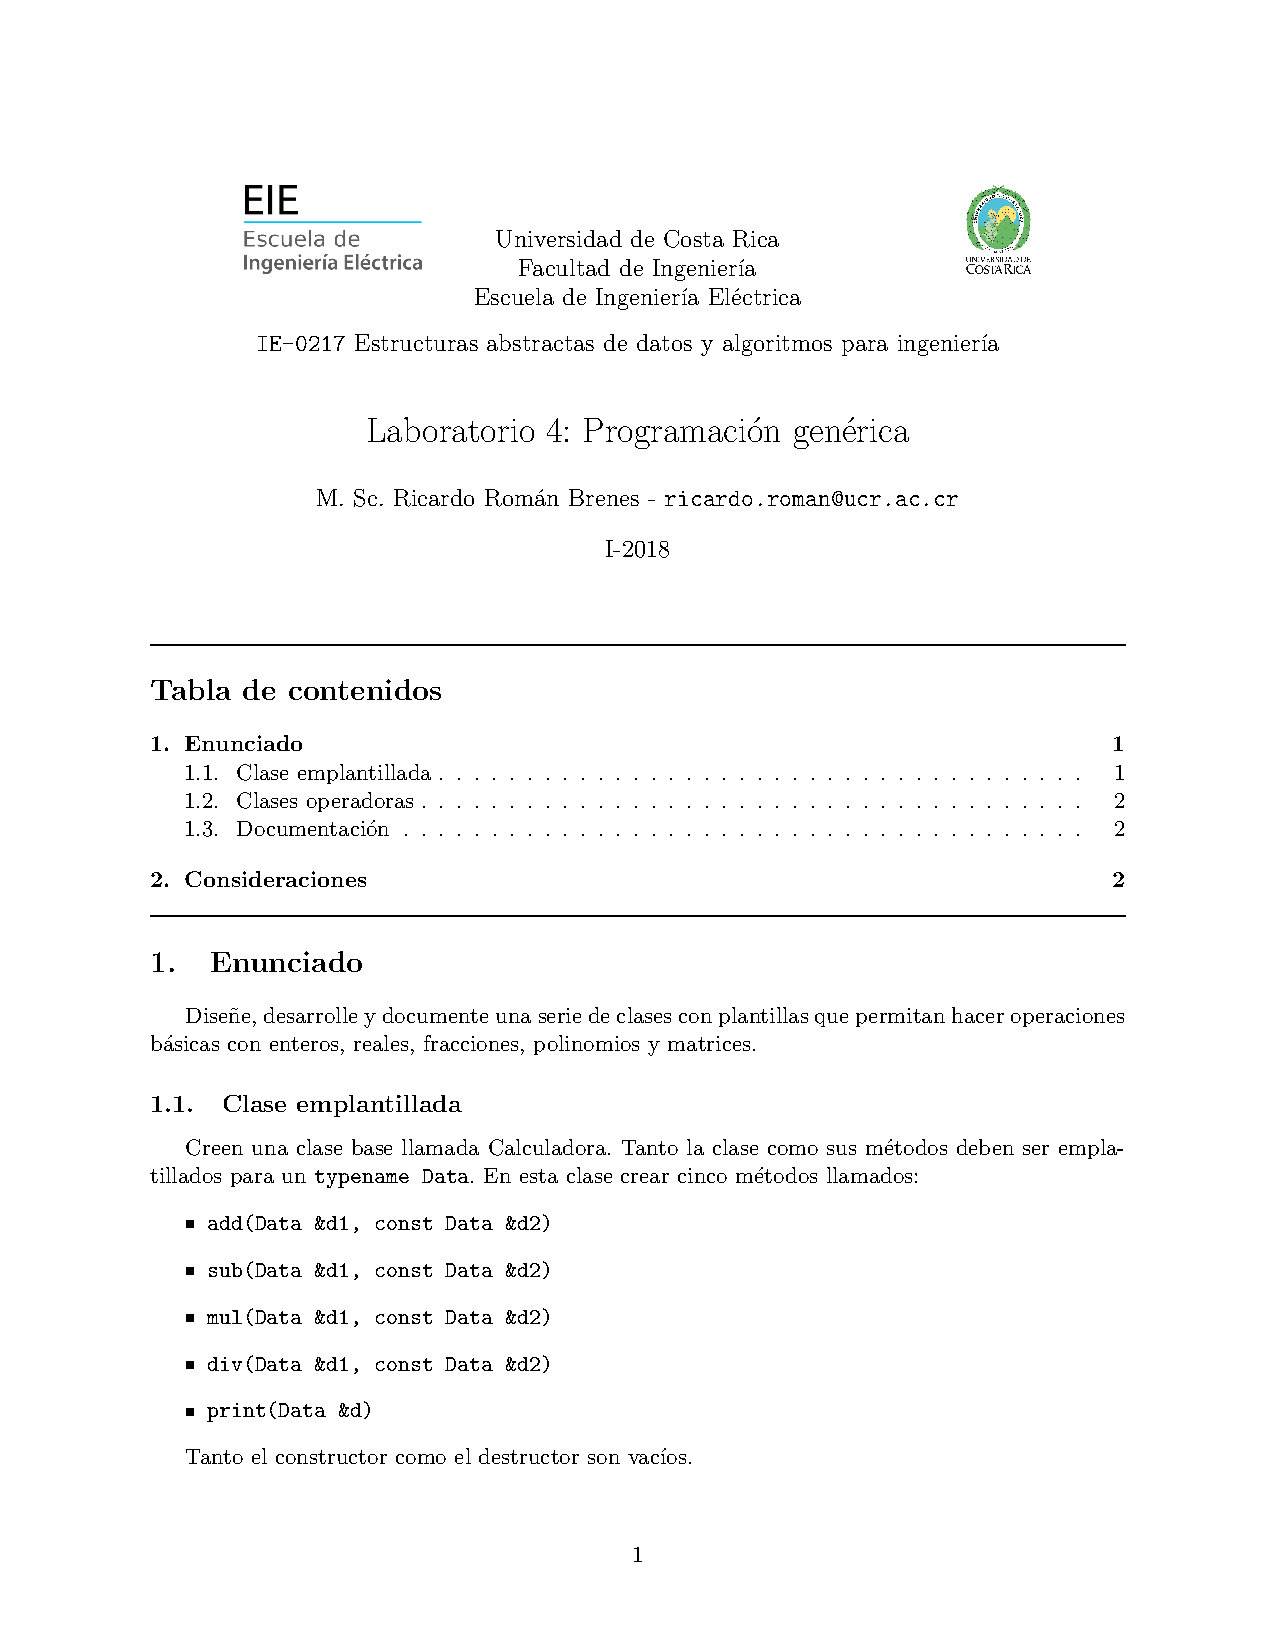
\includepdf[pages=1,pagecommand=\section{Enunciado}, scale=0.8]{enunciados/enun4} 
%\includepdf[pages=2,pagecommand={},scale=0.8]{enunciados/enun4}

%%%%%%%%%%%%%%%%%%%%%%%%%%%%%%%%%%%%%%%%%%%%%%%%%%%%%%%%%%%%%%
% --> SOLUCIÓN
%%%%%%%%%%%%%%%%%%%%%%%%%%%%%%%%%%%%%%%%%%%%%%%%%%%%%%%%%%%%%%
\section{Solución}


\begin{minted}[linenos,autogobble,bgcolor=bg,breaklines,fontsize=\footnotesize ]{c++}
#include <string>
#include <iostream>
using namespace std;

class FileUtil
{
  public:
  	FileUtil(string s, ios_base::openmode p);
  	~FileUtil();
  	string read();
  	string* readLines();
  	int write(string s);
  	int write(string* s, int n);
    void countNumberLines();
    int getNumberLines();
  private:
    //Numero de lineas.
    int numLines;
    //Dirección de lectura.
    string ruta;
    //Modo de lectura.
  	ios_base::openmode modo;
    //Linea leida.
    string line;
    //Puntero con la direccion del arreglo de las lineas leidas.
    string* lines;

};
\end{minted}



%%%%%%%%%%%%%%%%%%%%%%%%%%%%%%%%%%%%%%%%%%%%%%%%%%%%%%%%%%%%%%
% --> RESULTADOS
%%%%%%%%%%%%%%%%%%%%%%%%%%%%%%%%%%%%%%%%%%%%%%%%%%%%%%%%%%%%%%
\section{Resultados}



%%%%%%%%%%%%%%%%%%%%%%%%%%%%%%%%%%%%%%%%%%%%%%%%%%%%%%%%%%%%%%
% --> CONCLUSIONES
%%%%%%%%%%%%%%%%%%%%%%%%%%%%%%%%%%%%%%%%%%%%%%%%%%%%%%%%%%%%%%
\section{Conclusiones}


Como conclusiones se tiene que:

\begin{itemize}
\item 
\item 
\item 
\item 
\end{itemize}


%%%%%%%%%%%%%%%%%%%%%%%%%%%%%%%%%%%%%%%%%%%%%%%%%%%%%%%%%%%%%%
% --> BIBLIOGRAFIA
%%%%%%%%%%%%%%%%%%%%%%%%%%%%%%%%%%%%%%%%%%%%%%%%%%%%%%%%%%%%%%
\begin{thebibliography}{IEEE}
\bibitem{R1} Talens, S. \textbf{\textit{Curso de programación en C++}}. EUI (UPV) Valencia, 17 al 28 de Julio de 1995. 

\bibitem{R2} Raffo, E. \textbf{\textit{Programación genérica en C++, usando Metaprogramación}}. 2007. Sistemas de Informática. 
\end{thebibliography}



%%%%%%%%%%%%%%%%%%
%--> LABORATORIO 7
%%%%%%%%%%%%%%%%%%
%%%%%%%%%%%%%%%%%%%%%%%%%%%%%%%%%%%%%%%%%%%%%%%%%%%%%%%%%%%%%%%
% --> INTRODUCCIÓN
%%%%%%%%%%%%%%%%%%%%%%%%%%%%%%%%%%%%%%%%%%%%%%%%%%%%%%%%%%%%%%
\section{Introducción}


%%%%%%%%%%%%%%%%%%%%%%%%%%%%%%%%%%%%%%%%%%%%%%%%%%%%%%%%%%%%%%
% --> OBJETIVOS
%%%%%%%%%%%%%%%%%%%%%%%%%%%%%%%%%%%%%%%%%%%%%%%%%%%%%%%%%%%%%%
\subsection{Objetivos}



%%%%%%%%%%%%%%%%%%%%%%%%%%%%%%%%%%%%%%%%%%%%%%%%%%%%%%%%%%%%%%
% --> OBJETIVO GENERAL
%%%%%%%%%%%%%%%%%%%%%%%%%%%%%%%%%%%%%%%%%%%%%%%%%%%%%%%%%%%%%%
\subsubsection{Objetivo General}
\begin{itemize}
\item 
\end{itemize}

%%%%%%%%%%%%%%%%%%%%%%%%%%%%%%%%%%%%%%%%%%%%%%%%%%%%%%%%%%%%%%
% --> OBJETIVOS ESPECÍFICOS
%%%%%%%%%%%%%%%%%%%%%%%%%%%%%%%%%%%%%%%%%%%%%%%%%%%%%%%%%%%%%%
\subsubsection{Objetivos Específicos}
\begin{itemize}
\item 
\item 
\item 
\item
\item 
\end{itemize}

%%%%%%%%%%%%%%%%%%%%%%%%%%%%%%%%%%%%%%%%%%%%%%%%%%%%%%%%%%%%%%
% --> ENUNCIADO
%%%%%%%%%%%%%%%%%%%%%%%%%%%%%%%%%%%%%%%%%%%%%%%%%%%%%%%%%%%%%%
%\newpage

%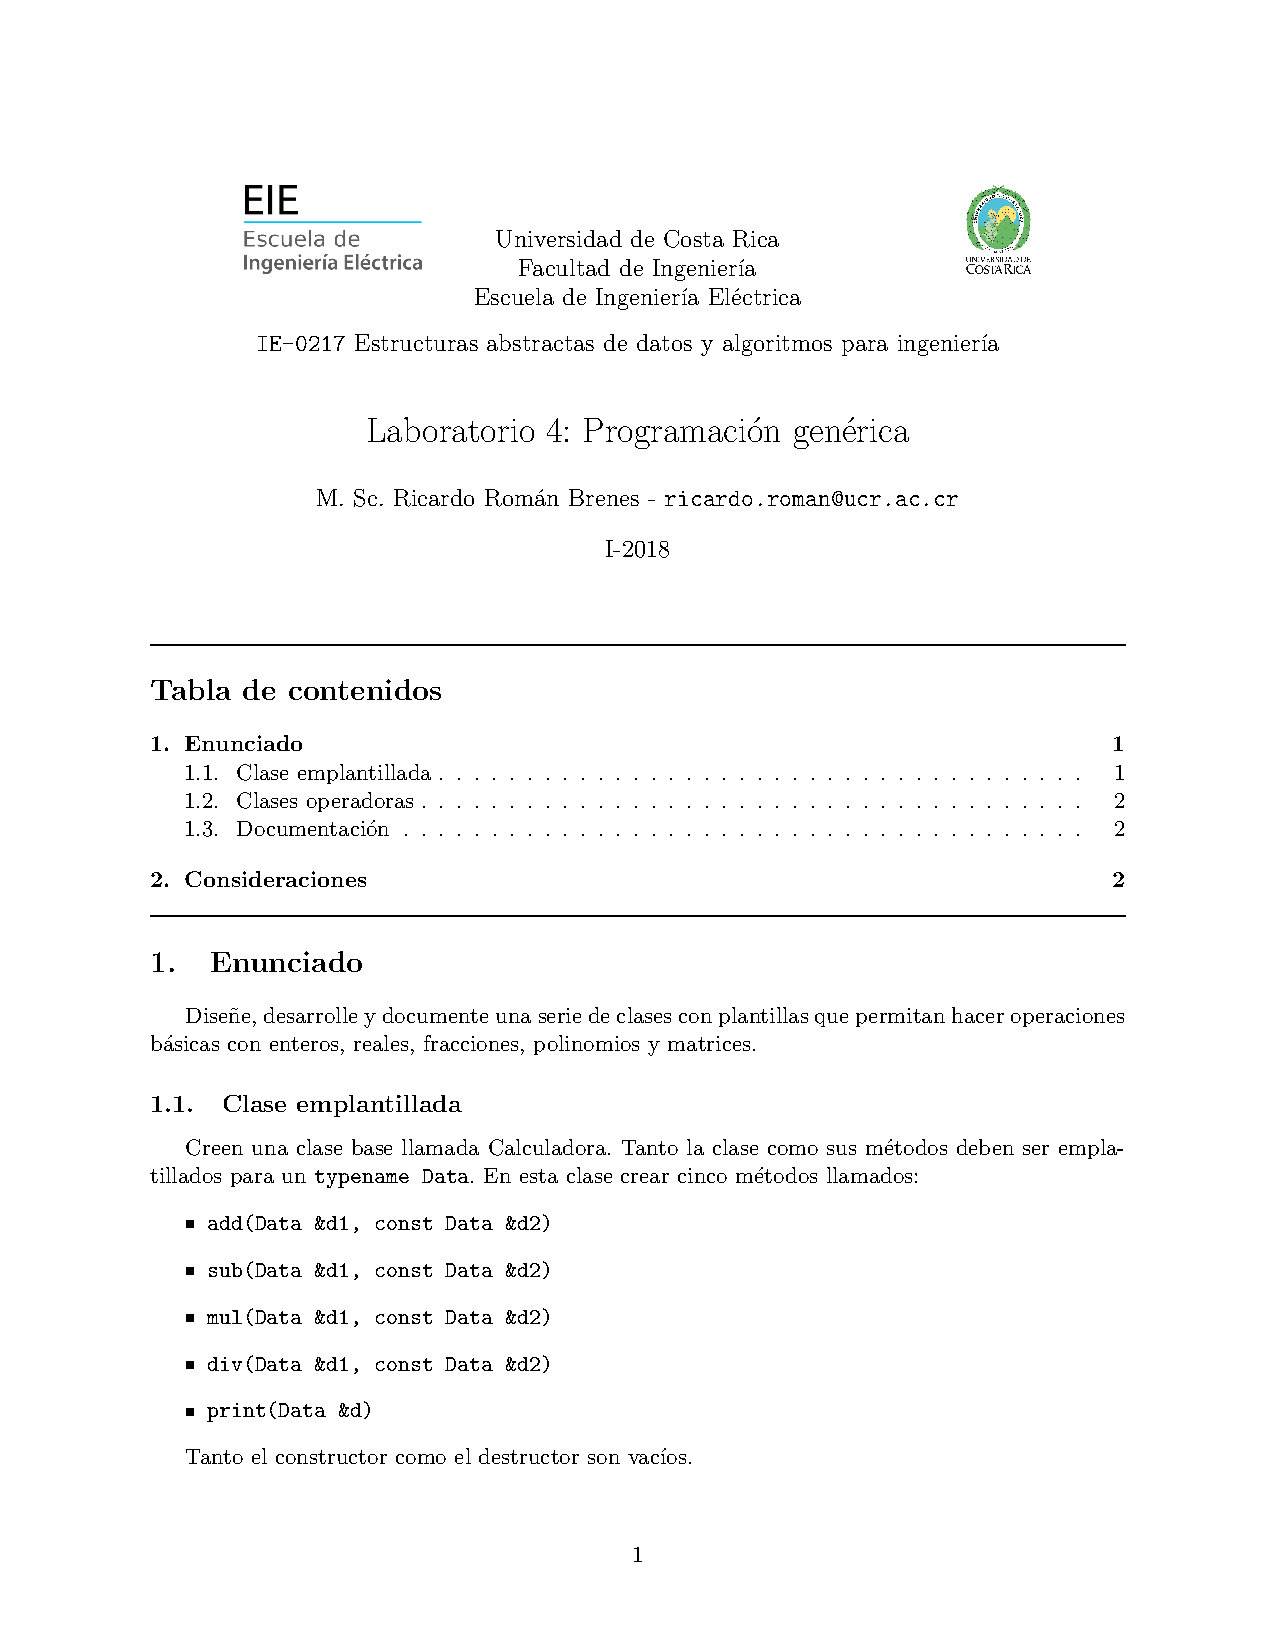
\includepdf[pages=1,pagecommand=\section{Enunciado}, scale=0.8]{enunciados/enun4} 
%\includepdf[pages=2,pagecommand={},scale=0.8]{enunciados/enun4}

%%%%%%%%%%%%%%%%%%%%%%%%%%%%%%%%%%%%%%%%%%%%%%%%%%%%%%%%%%%%%%
% --> SOLUCIÓN
%%%%%%%%%%%%%%%%%%%%%%%%%%%%%%%%%%%%%%%%%%%%%%%%%%%%%%%%%%%%%%
\section{Solución}


\begin{minted}[linenos,autogobble,bgcolor=bg,breaklines,fontsize=\footnotesize ]{c++}
#include <string>
#include <iostream>
using namespace std;

class FileUtil
{
  public:
  	FileUtil(string s, ios_base::openmode p);
  	~FileUtil();
  	string read();
  	string* readLines();
  	int write(string s);
  	int write(string* s, int n);
    void countNumberLines();
    int getNumberLines();
  private:
    //Numero de lineas.
    int numLines;
    //Dirección de lectura.
    string ruta;
    //Modo de lectura.
  	ios_base::openmode modo;
    //Linea leida.
    string line;
    //Puntero con la direccion del arreglo de las lineas leidas.
    string* lines;

};
\end{minted}



%%%%%%%%%%%%%%%%%%%%%%%%%%%%%%%%%%%%%%%%%%%%%%%%%%%%%%%%%%%%%%
% --> RESULTADOS
%%%%%%%%%%%%%%%%%%%%%%%%%%%%%%%%%%%%%%%%%%%%%%%%%%%%%%%%%%%%%%
\section{Resultados}



%%%%%%%%%%%%%%%%%%%%%%%%%%%%%%%%%%%%%%%%%%%%%%%%%%%%%%%%%%%%%%
% --> CONCLUSIONES
%%%%%%%%%%%%%%%%%%%%%%%%%%%%%%%%%%%%%%%%%%%%%%%%%%%%%%%%%%%%%%
\section{Conclusiones}


Como conclusiones se tiene que:

\begin{itemize}
\item 
\item 
\item 
\item 
\end{itemize}


%%%%%%%%%%%%%%%%%%%%%%%%%%%%%%%%%%%%%%%%%%%%%%%%%%%%%%%%%%%%%%
% --> BIBLIOGRAFIA
%%%%%%%%%%%%%%%%%%%%%%%%%%%%%%%%%%%%%%%%%%%%%%%%%%%%%%%%%%%%%%
\begin{thebibliography}{IEEE}
\bibitem{R1} Talens, S. \textbf{\textit{Curso de programación en C++}}. EUI (UPV) Valencia, 17 al 28 de Julio de 1995. 

\bibitem{R2} Raffo, E. \textbf{\textit{Programación genérica en C++, usando Metaprogramación}}. 2007. Sistemas de Informática. 
\end{thebibliography}



%%%%%%%%%%%%%%%%%%
%--> LABORATORIO 8
%%%%%%%%%%%%%%%%%%
%%%%%%%%%%%%%%%%%%%%%%%%%%%%%%%%%%%%%%%%%%%%%%%%%%%%%%%%%%%%%%%
% --> INTRODUCCIÓN
%%%%%%%%%%%%%%%%%%%%%%%%%%%%%%%%%%%%%%%%%%%%%%%%%%%%%%%%%%%%%%
\section{Introducción}


%%%%%%%%%%%%%%%%%%%%%%%%%%%%%%%%%%%%%%%%%%%%%%%%%%%%%%%%%%%%%%
% --> OBJETIVOS
%%%%%%%%%%%%%%%%%%%%%%%%%%%%%%%%%%%%%%%%%%%%%%%%%%%%%%%%%%%%%%
\subsection{Objetivos}



%%%%%%%%%%%%%%%%%%%%%%%%%%%%%%%%%%%%%%%%%%%%%%%%%%%%%%%%%%%%%%
% --> OBJETIVO GENERAL
%%%%%%%%%%%%%%%%%%%%%%%%%%%%%%%%%%%%%%%%%%%%%%%%%%%%%%%%%%%%%%
\subsubsection{Objetivo General}
\begin{itemize}
\item 
\end{itemize}

%%%%%%%%%%%%%%%%%%%%%%%%%%%%%%%%%%%%%%%%%%%%%%%%%%%%%%%%%%%%%%
% --> OBJETIVOS ESPECÍFICOS
%%%%%%%%%%%%%%%%%%%%%%%%%%%%%%%%%%%%%%%%%%%%%%%%%%%%%%%%%%%%%%
\subsubsection{Objetivos Específicos}
\begin{itemize}
\item 
\item 
\item 
\item
\item 
\end{itemize}

%%%%%%%%%%%%%%%%%%%%%%%%%%%%%%%%%%%%%%%%%%%%%%%%%%%%%%%%%%%%%%
% --> ENUNCIADO
%%%%%%%%%%%%%%%%%%%%%%%%%%%%%%%%%%%%%%%%%%%%%%%%%%%%%%%%%%%%%%
%\newpage

%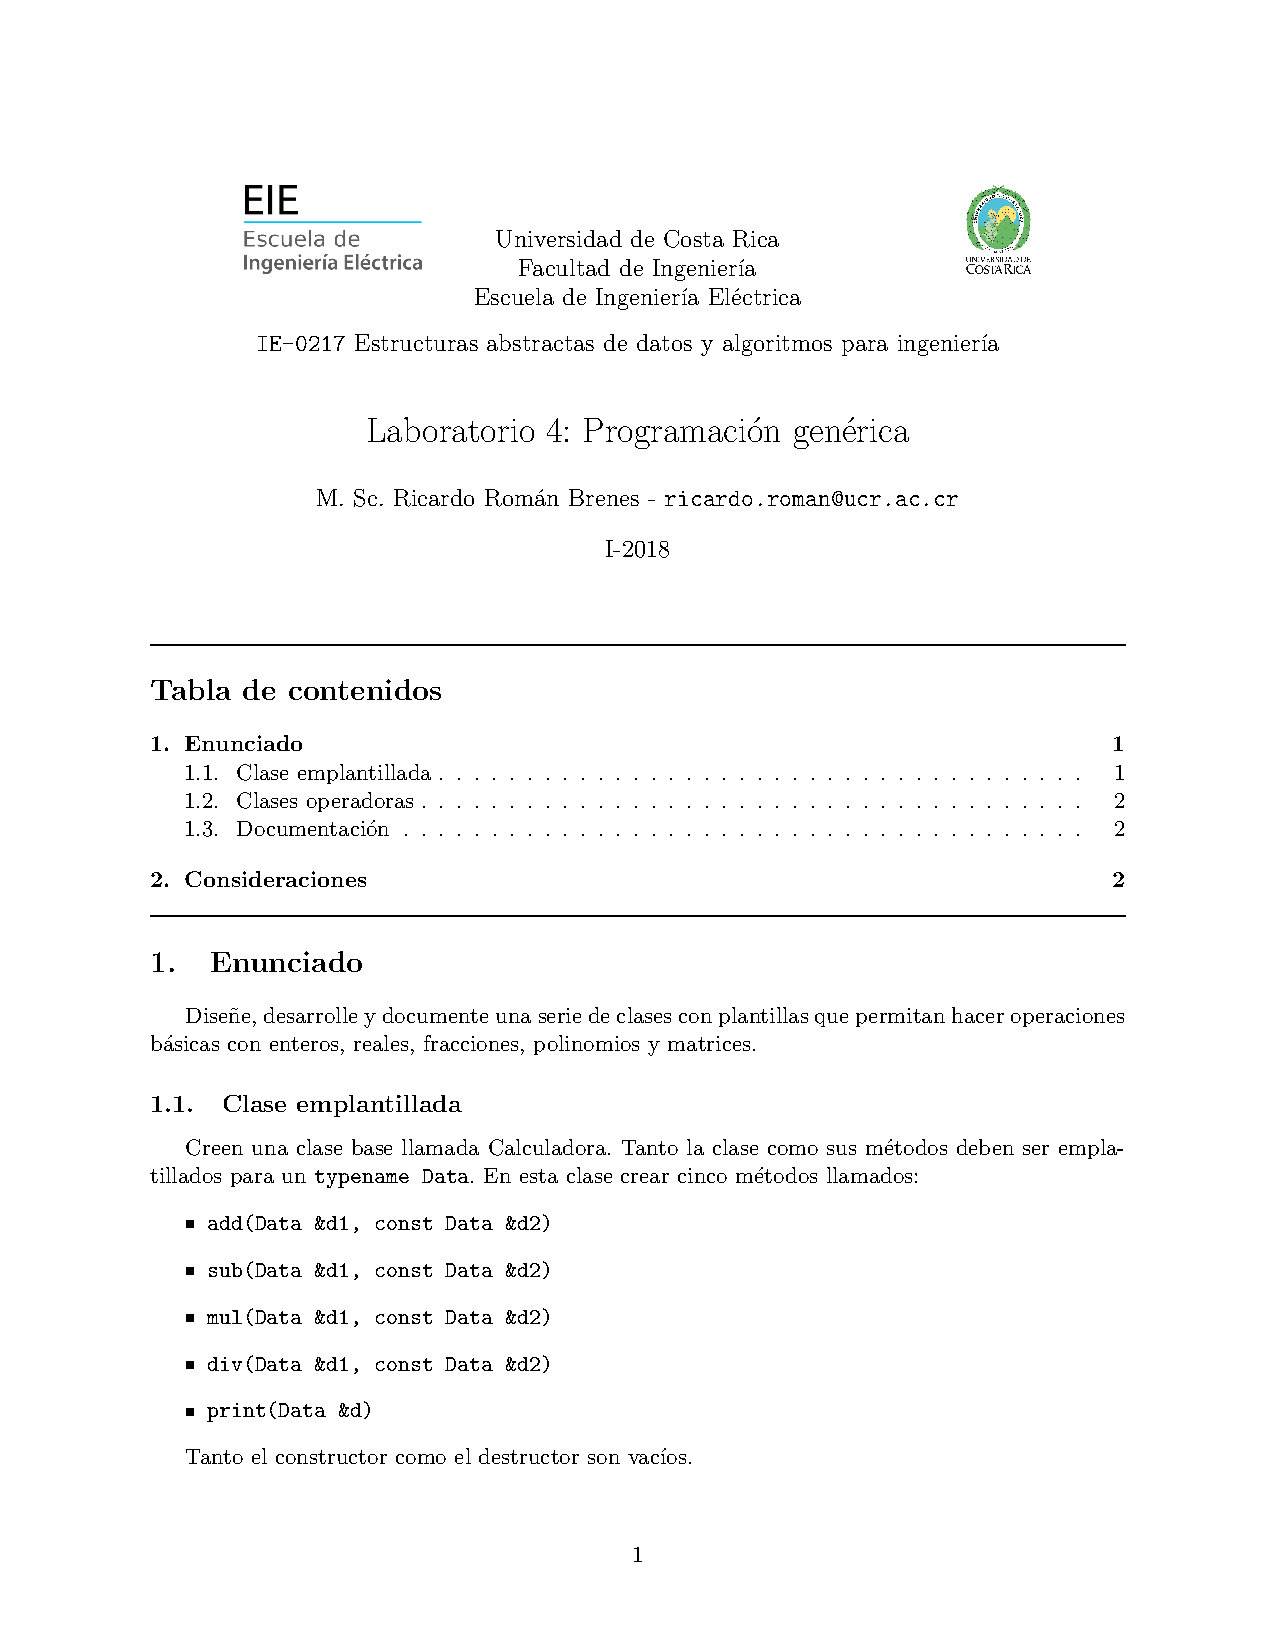
\includepdf[pages=1,pagecommand=\section{Enunciado}, scale=0.8]{enunciados/enun4} 
%\includepdf[pages=2,pagecommand={},scale=0.8]{enunciados/enun4}

%%%%%%%%%%%%%%%%%%%%%%%%%%%%%%%%%%%%%%%%%%%%%%%%%%%%%%%%%%%%%%
% --> SOLUCIÓN
%%%%%%%%%%%%%%%%%%%%%%%%%%%%%%%%%%%%%%%%%%%%%%%%%%%%%%%%%%%%%%
\section{Solución}


\begin{minted}[linenos,autogobble,bgcolor=bg,breaklines,fontsize=\footnotesize ]{c++}
#include <string>
#include <iostream>
using namespace std;

class FileUtil
{
  public:
  	FileUtil(string s, ios_base::openmode p);
  	~FileUtil();
  	string read();
  	string* readLines();
  	int write(string s);
  	int write(string* s, int n);
    void countNumberLines();
    int getNumberLines();
  private:
    //Numero de lineas.
    int numLines;
    //Dirección de lectura.
    string ruta;
    //Modo de lectura.
  	ios_base::openmode modo;
    //Linea leida.
    string line;
    //Puntero con la direccion del arreglo de las lineas leidas.
    string* lines;

};
\end{minted}



%%%%%%%%%%%%%%%%%%%%%%%%%%%%%%%%%%%%%%%%%%%%%%%%%%%%%%%%%%%%%%
% --> RESULTADOS
%%%%%%%%%%%%%%%%%%%%%%%%%%%%%%%%%%%%%%%%%%%%%%%%%%%%%%%%%%%%%%
\section{Resultados}



%%%%%%%%%%%%%%%%%%%%%%%%%%%%%%%%%%%%%%%%%%%%%%%%%%%%%%%%%%%%%%
% --> CONCLUSIONES
%%%%%%%%%%%%%%%%%%%%%%%%%%%%%%%%%%%%%%%%%%%%%%%%%%%%%%%%%%%%%%
\section{Conclusiones}


Como conclusiones se tiene que:

\begin{itemize}
\item 
\item 
\item 
\item 
\end{itemize}


%%%%%%%%%%%%%%%%%%%%%%%%%%%%%%%%%%%%%%%%%%%%%%%%%%%%%%%%%%%%%%
% --> BIBLIOGRAFIA
%%%%%%%%%%%%%%%%%%%%%%%%%%%%%%%%%%%%%%%%%%%%%%%%%%%%%%%%%%%%%%
\begin{thebibliography}{IEEE}
\bibitem{R1} Talens, S. \textbf{\textit{Curso de programación en C++}}. EUI (UPV) Valencia, 17 al 28 de Julio de 1995. 

\bibitem{R2} Raffo, E. \textbf{\textit{Programación genérica en C++, usando Metaprogramación}}. 2007. Sistemas de Informática. 
\end{thebibliography}



%\newpage
%\bibliographystyle{plain}
%\bibliography{bibliography}



\end{document}
